\documentclass[a4paper,12pt]{article}
\usepackage{graphicx}
\usepackage{amsmath, amssymb}
\usepackage{float}
\usepackage{subcaption}
\usepackage{siunitx}
\usepackage{hyperref}
\usepackage{circuitikz}

\title{\textbf{Second order filters}}
\author{Sai Akhila - EE24BTECH11055 \\Sai Akshita - EE24BTECH11054}
\date{\today}
\begin{document}
\maketitle

\section{Objective:}
\begin{itemize}
    \item To design and implement a bandpass filter using separate Sallen-Key Low Pass Filter (LPF) and High Pass Filter (HPF).
    \item To analyze and compare the frequency response of LPF, HPF, and the final bandpass filter.
    \item To plot the magnitude response (gain vs. frequency) of all three filters.
\end{itemize}

\section{Components and Equipment Required:}
\begin{itemize}
\item  Operational Amplifiers (e.g., TL074, TL081, or LM358)
\item  Resistors: R1, R2, R3, R4 (in k$\Omega$)
\item  Capacitors: C1, C2, C3, C4 (in nF)
\item  Function Generator
\item  Oscilloscope or Spectrum Analyzer
\item  DC Power Supply (±12V)
\item  Breadboard and connecting wires
\end{itemize}


\section{Role of Op-Amp in Sallen-Key Filters:}
\begin{itemize}
    \item Helps in Amplification of the output signal.
    \item The high input impedance and low output impedance of an op-amp prevent loading effects.
    \item Allows better control over cutoff frequency, Q-factor, and bandwidth compared to passive filters.
    \item Op-amps ensure better linearity and stable frequency response, reducing signal distortion.
\end{itemize}

\section{Types of Filter Designs:}
\begin{itemize}
    \item \textbf{Butterworth Filter:} Maximally flat frequency response ()
    \item \textbf{Chebyshev Filter:} Faster roll-off than Butterworth but introduces ripples.
    \item \textbf{Bessel Filter:} Best for preserving waveform shape (constant group delay).
\end{itemize}


\section{Types of Filters }
\subsection{Sallen-Key Low Pass Filter}
The Sallen-Key low-pass filter is a second-order active filter that allows low-frequency signals to pass while attenuating higher-frequency signals. It consists of an op-amp, two resistors, and two capacitors arranged in the given specific topology.\\\\

\begin{figure}[H]
    \centering
    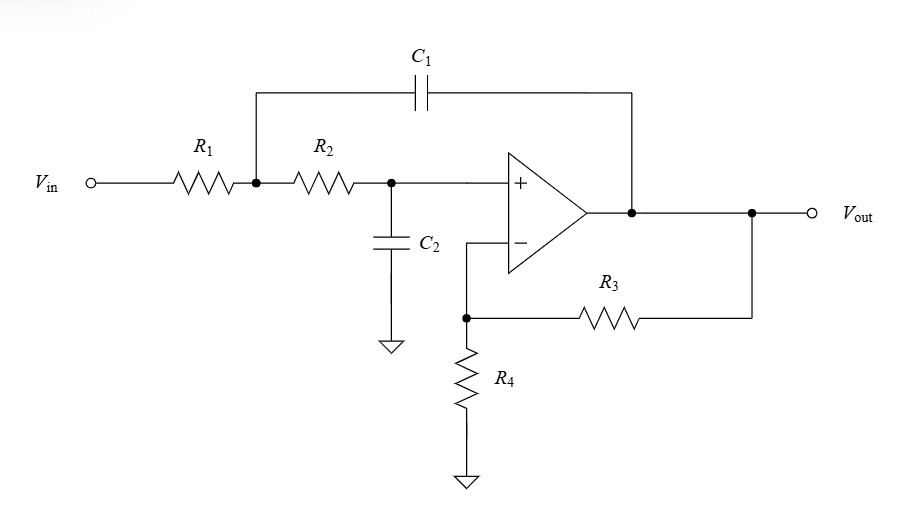
\includegraphics[width=0.5\textwidth]{fig/lpc.jpeg}
    \caption{Sallen-Key Low pass filter}
    \label{fig:yourlabel}
\end{figure}

\textbf{Working Principle:}
\begin{itemize}
    \item When low-frequency signals are given as input to the circuit, the impedance of the capacitors $(\frac{1}{\omega C})$ is high, resulting in open- wire behaviour of the capacitor branch. This ensures that the signal is passed  that with minimal attenuation. 
    \item When high-frequency signals are given as input to the circuit, the impedance of the capacitors $(\frac{1}{\omega C})$ is low, resuiting in lower impedance behaviour of the capacitor branch. Thus, more amount of current flows in to the branch and hence, the signal is not reached to $V_{out}$.
    \item The input signal (Vin) passes through R1 and C1, forming the first stage of filtering.
    \item R2 and C2 create a second filtering stage before the op-amp.
    \item The op-amp acts as a buffer to prevent loading effects and maintain stability.
    \item The resistors R1 and R2 form a voltage divider with C1 and C2 and define the cutoff frequency.
    \item R3 and R4 allow gain adjustment.
    \item C1, also known as Feedback capacitor, Works with R1 and R2 to determine the filter's frequency response and provides negative feedback to the op-amp, improving stability.
    \item C2 Forms a low-pass network with R2.
     \item Transfer function of the filter is $H(s) = \frac{K}{s^2 + \frac{\omega_c}{Q}s + \omega_c^2}$, where K is the gain.
     \item Quality factor is $Q = \frac{\sqrt{R_1 R_2 C_1 C_2}}{R_1 + R_2}$
    \item At cutoff-frequency, the output voltage drops to $70.7\%$(-3dB) of the input voltage if r1=r2=r and c1=c2=c.(optional)
    \item The cutoff Frequency is given by$  f_c=\frac{1}{2\pi\sqrt{ R_1R_2C_1C_2}}$
\end{itemize}

\subsection{Sallen-Key High Pass Filter}
The Sallen-Key high-pass filter is a second-order active filter that allows high-frequency signals to pass while attenuating lower-frequency signals. It consists of an op-amp, two resistors, and two capacitors arranged in the given specific topology.\\\\
\begin{figure}[H]
    \centering
    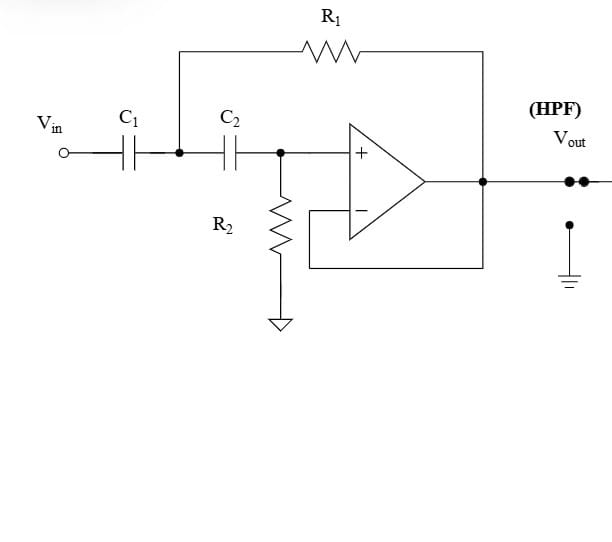
\includegraphics[width=0.5\textwidth]{fig/hpc.jpeg}
    \caption{Sallen-Key High pass filter}
    \label{fig:yourlabel}
\end{figure}
\textbf{Working Principle:}
\begin{itemize}
    \item When high-frequency signals are given as input to the circuit, the impedance of the capacitors $(\frac{1}{\omega C})$ is low, resulting in lower impedance behaviour of the capacitor branch. This ensures that the signal is passed  that with minimal attenuation. 
    \item When low-frequency signals are given as input to the circuit, the impedance of the capacitors $(\frac{1}{\omega C})$ is high, resuiting in open-wire behaviour of the capacitor branch. Thus, less amount of current flows in to the branch and hence, the signal is not reached to $V_{out}$.
    \item C1 (Input Capacitor) blocks low frequencies and allows high frequencies to pass.
    \item C2 (Feedback Capacitor) Shapes the frequency response by interacting with the op-amp’s feedback loop.
    \item The cutoff frequency is given by $f_c=\frac{1}{2\pi\sqrt{ R_1R_2C_1C_2}}$
    \item gain is given by $K=1+\frac{R_3}{R_4}$
    \item At cutoff-frequency, the output voltage drops to $70.7\%$(-3dB) of the input voltage if r1=r2=r and c1=c2=c.
\end{itemize}


subsection{Sallen-Key Band Pass Filter}
A Butter-worth band-pass filter is a type of electronic filter that passes frequencies within a certain range and attenuates frequencies outside that range. The Butterworth bandpass filter is typically constructed by cascading a low-pass and a high-pass filter.\\\\
\begin{figure}[H]
    \centering
    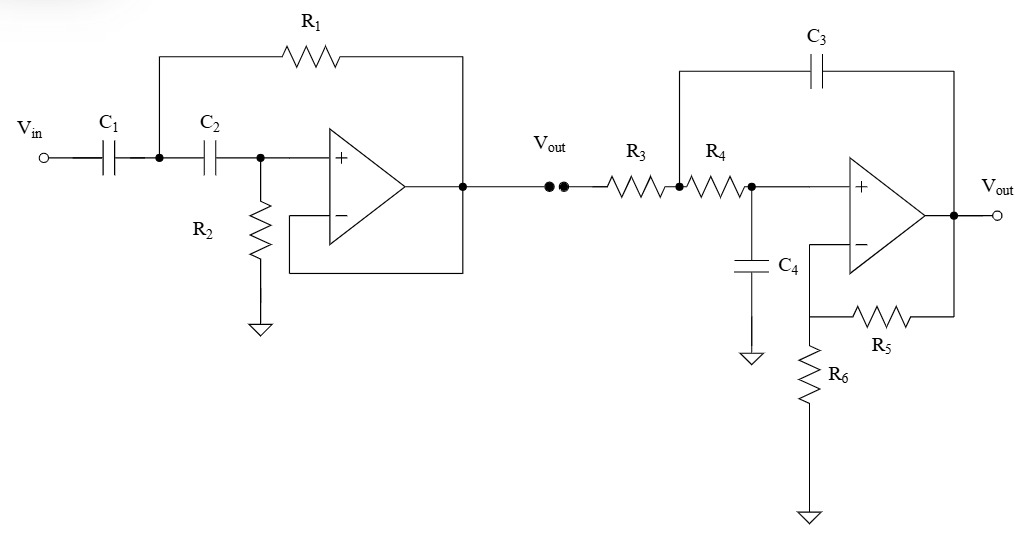
\includegraphics[width=0.8\textwidth]{fig/bpc.jpeg}
    \caption{Circuit Diagram}
    \label{fig:your-label}
\end{figure}
\textbf{Working Principle:}
\begin{itemize}
    \item The bandpass filter is typically constructed by cascading a high-pass and a low-pass Sallen-Key filter stage.
    \item The lower cutoff frequency $(f_L)$ is determined by the high-pass section, while the upper cutoff frequency $(f_H)$ is set by the low-pass section.
    \item When input frequencies are between $f_L$ and $f_H$, the filter allows them to pass with minimal attenuation.
    \item For frequencies below $f_L$, the high-pass section attenuates the signal, while the low-pass section has little effect.
    \item For frequencies above $f_H$, the low-pass section attenuates the signal, while the high-pass section has minimal impact.
    \item The center frequency $(f_c)$ of the bandpass filter is the geometric mean of $f_L$ and $f_H$, given by: $f_c = \sqrt{(f_L \times f_H)}$
    \item The bandwidth (BW) is defined as the difference between the upper and lower cutoff frequencies: $BW = f_H - f_L$
    \item The quality factor (Q) of the bandpass filter is given by: $Q = f_c / BW$
    \item The transfer function of the bandpass filter is the product of the high-pass and low-pass transfer functions:
    $$H(s)=\frac{Ks}{s^2+\frac{\omega _cs}{Q}+\omega _c ^2}$$,
    where K is the gain, $\omega _c$ is the center frequency in radians/second, and Q is the quality factor. 
    \item The gain at the center frequency is determined by the Q factor and cannot be set independently as in low-pass or high-pass filters.
\end{itemize}

\section{Procedure and Observations}
\subsection{Low-Pass Filter}
\begin{enumerate}
    \item Assemble the Sallen-key LPF circuit on the breadboard.
    \item Use the function Generator to apply a sine wave.
    \item Vary the input frequency and measure the output voltage.
    \item Record gain values for different frequencies.
    \item Plot gain vs. frequency (Bode plot).
\end{enumerate}
\subsubsection{Observations}

\begin{figure}[H]
    \centering
    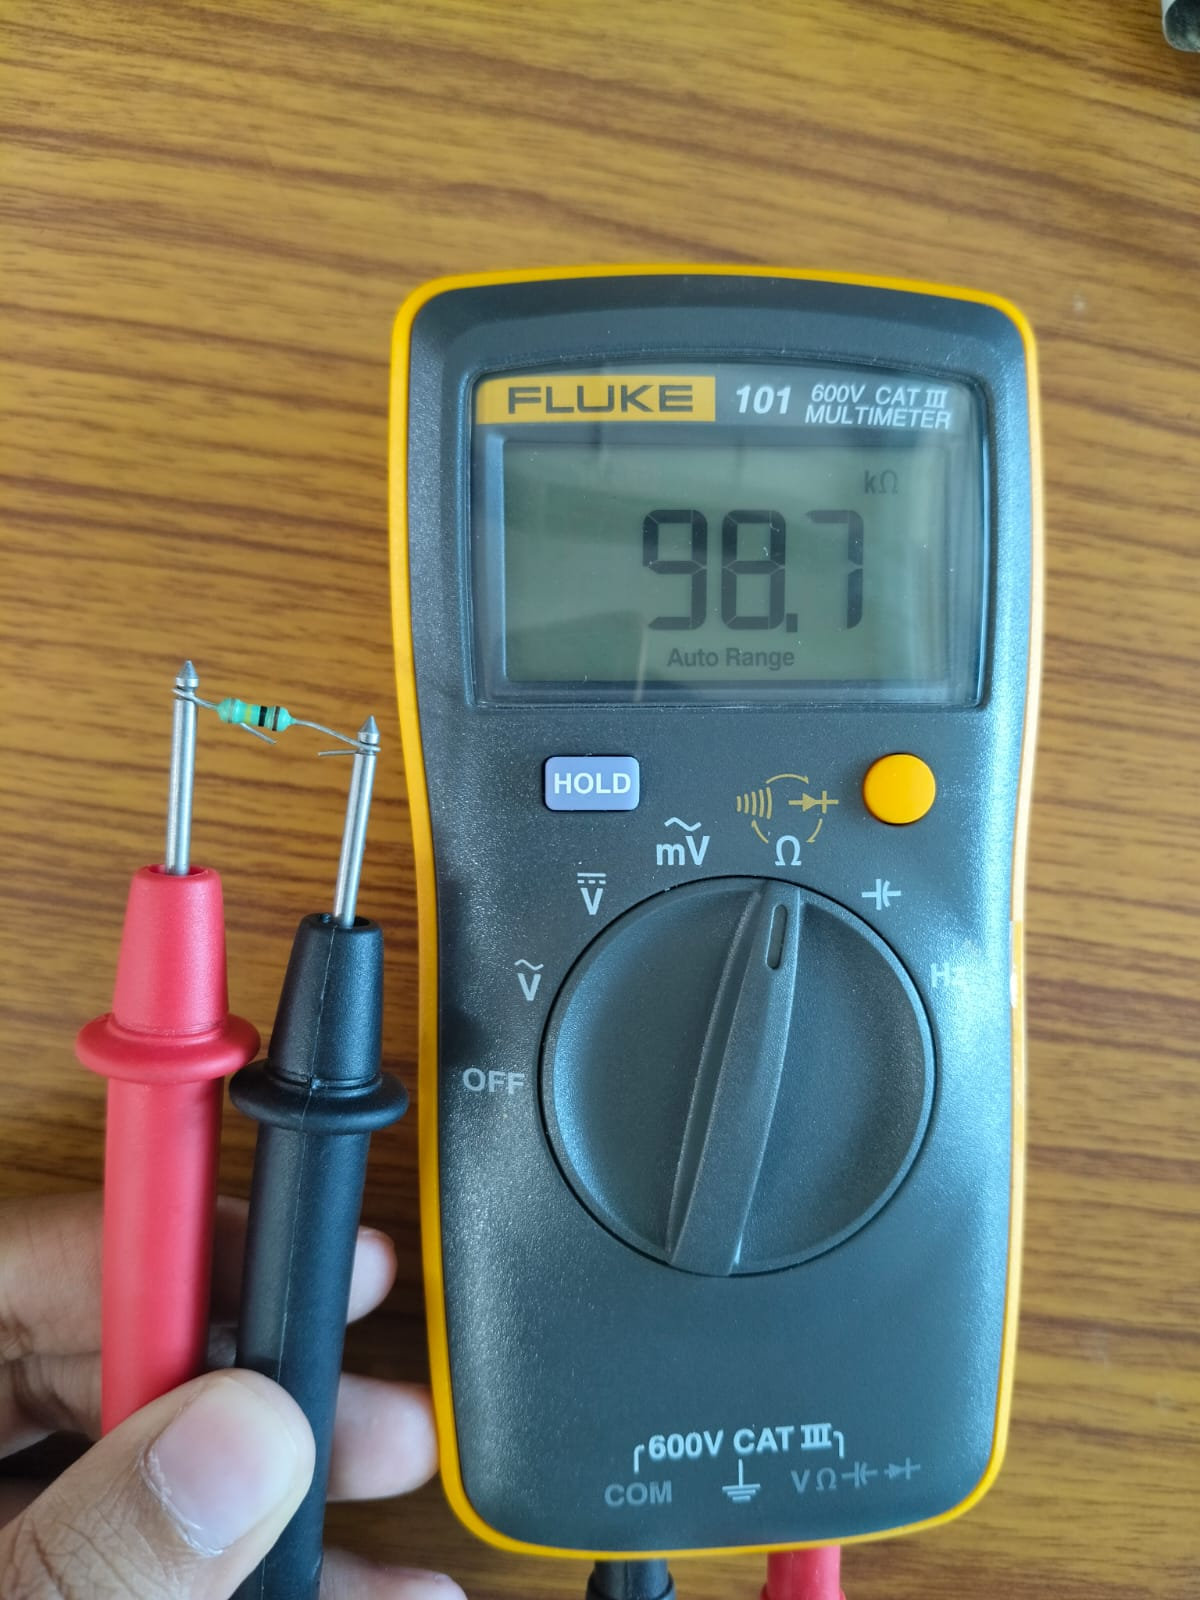
\includegraphics[width=0.8\textwidth]{fig/m/100kohm.jpeg}
    \caption{Resistance}
    \label{fig:your-label}
\end{figure}

\begin{figure}[H]
    \centering
    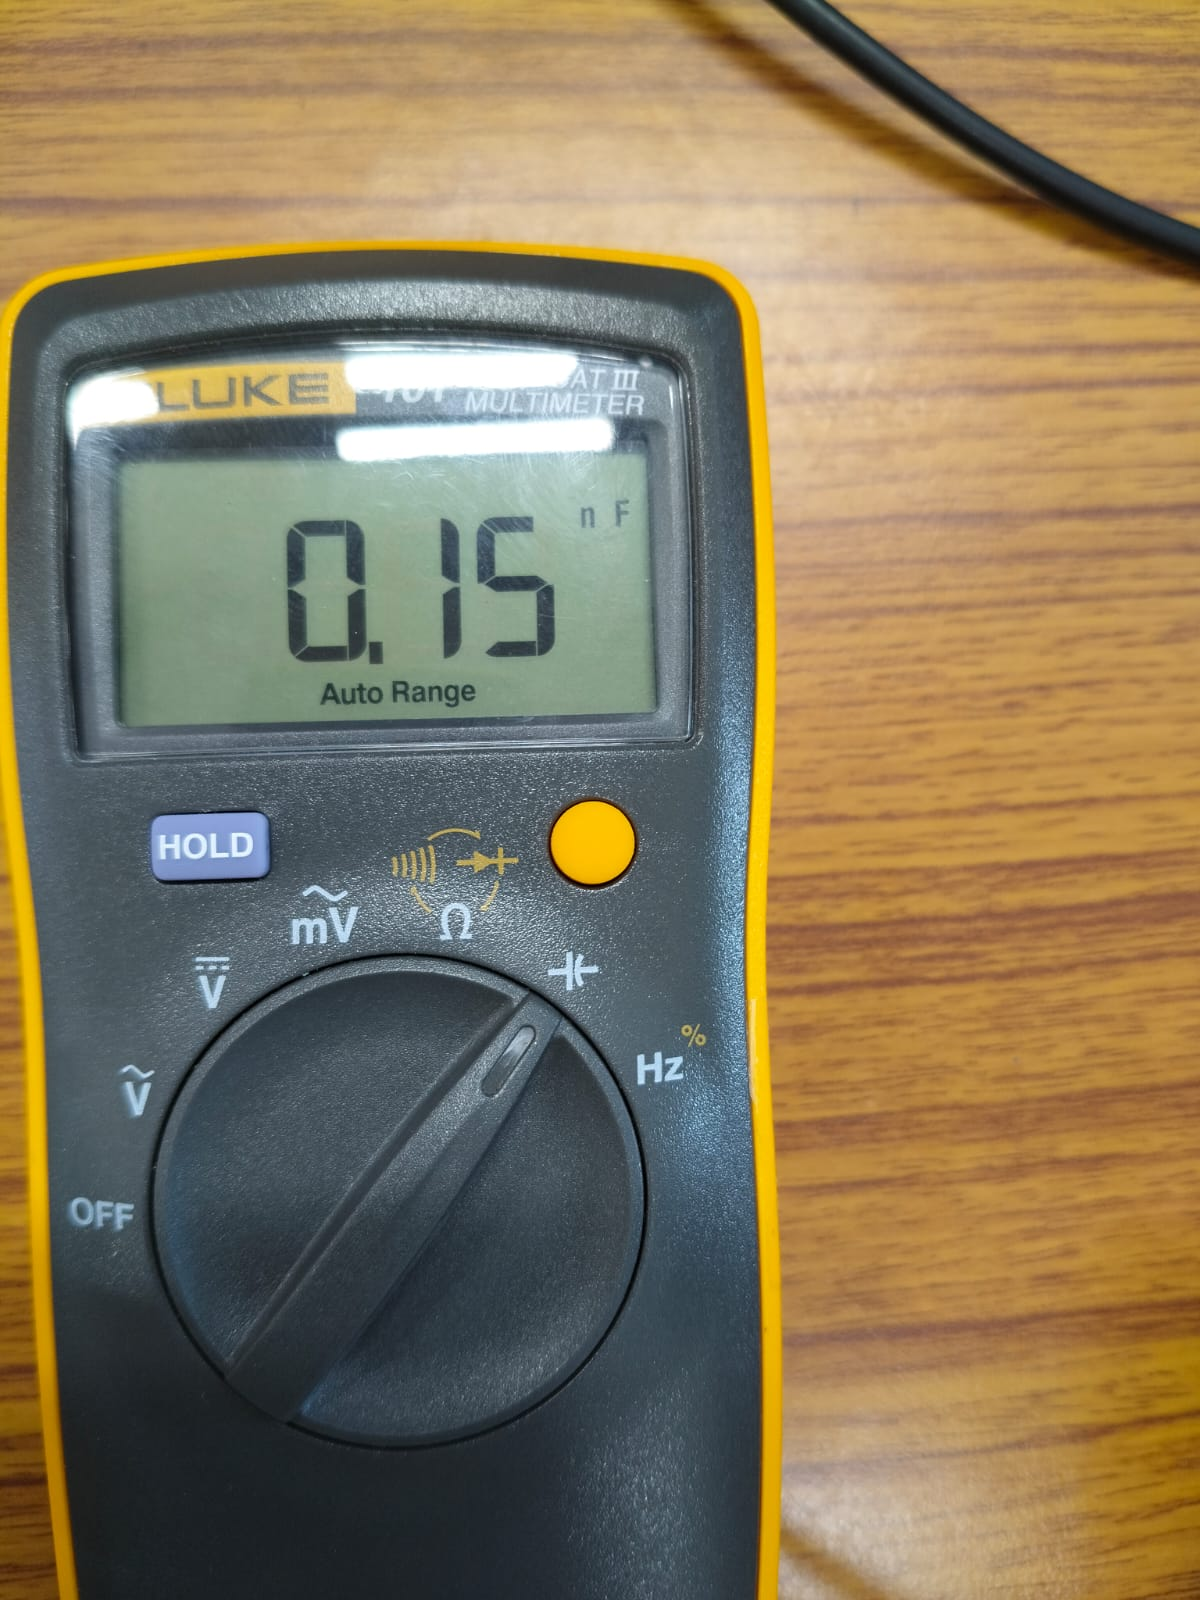
\includegraphics[width=0.8\textwidth]{fig/m/nf.jpeg}
    \caption{Resistance}
    \label{fig:your-label}
\end{figure}


The table below shows a comparison between measured values of $V_{pp}$ and Theoretically expected ones. 
\begin{table}[H]
\centering
\begin{tabular}{|c|c|c|}
\hline
\textbf{Frequency(in Hz)} & \textbf{Measured Value}  \\
\hline
10 & 11.2   \\
200 & 11.8     \\
300 & 11.6   \\
1894 & 8.321   \\
2000 & 22.20   \\
3000 & 10.4  \\
5000 & 4.96  \\
6000 & 3.04   \\
7000 & 2.08  \\
8000 & 1.58  \\
9000 & 1.201  \\
10000 & 0.96  \\

\hline
\end{tabular}
\caption{Measured vs Theoretical Values}
\end{table}



\begin{figure}[H]
    \centering
    \begin{minipage}[b]{0.45\textwidth}
        \centering
        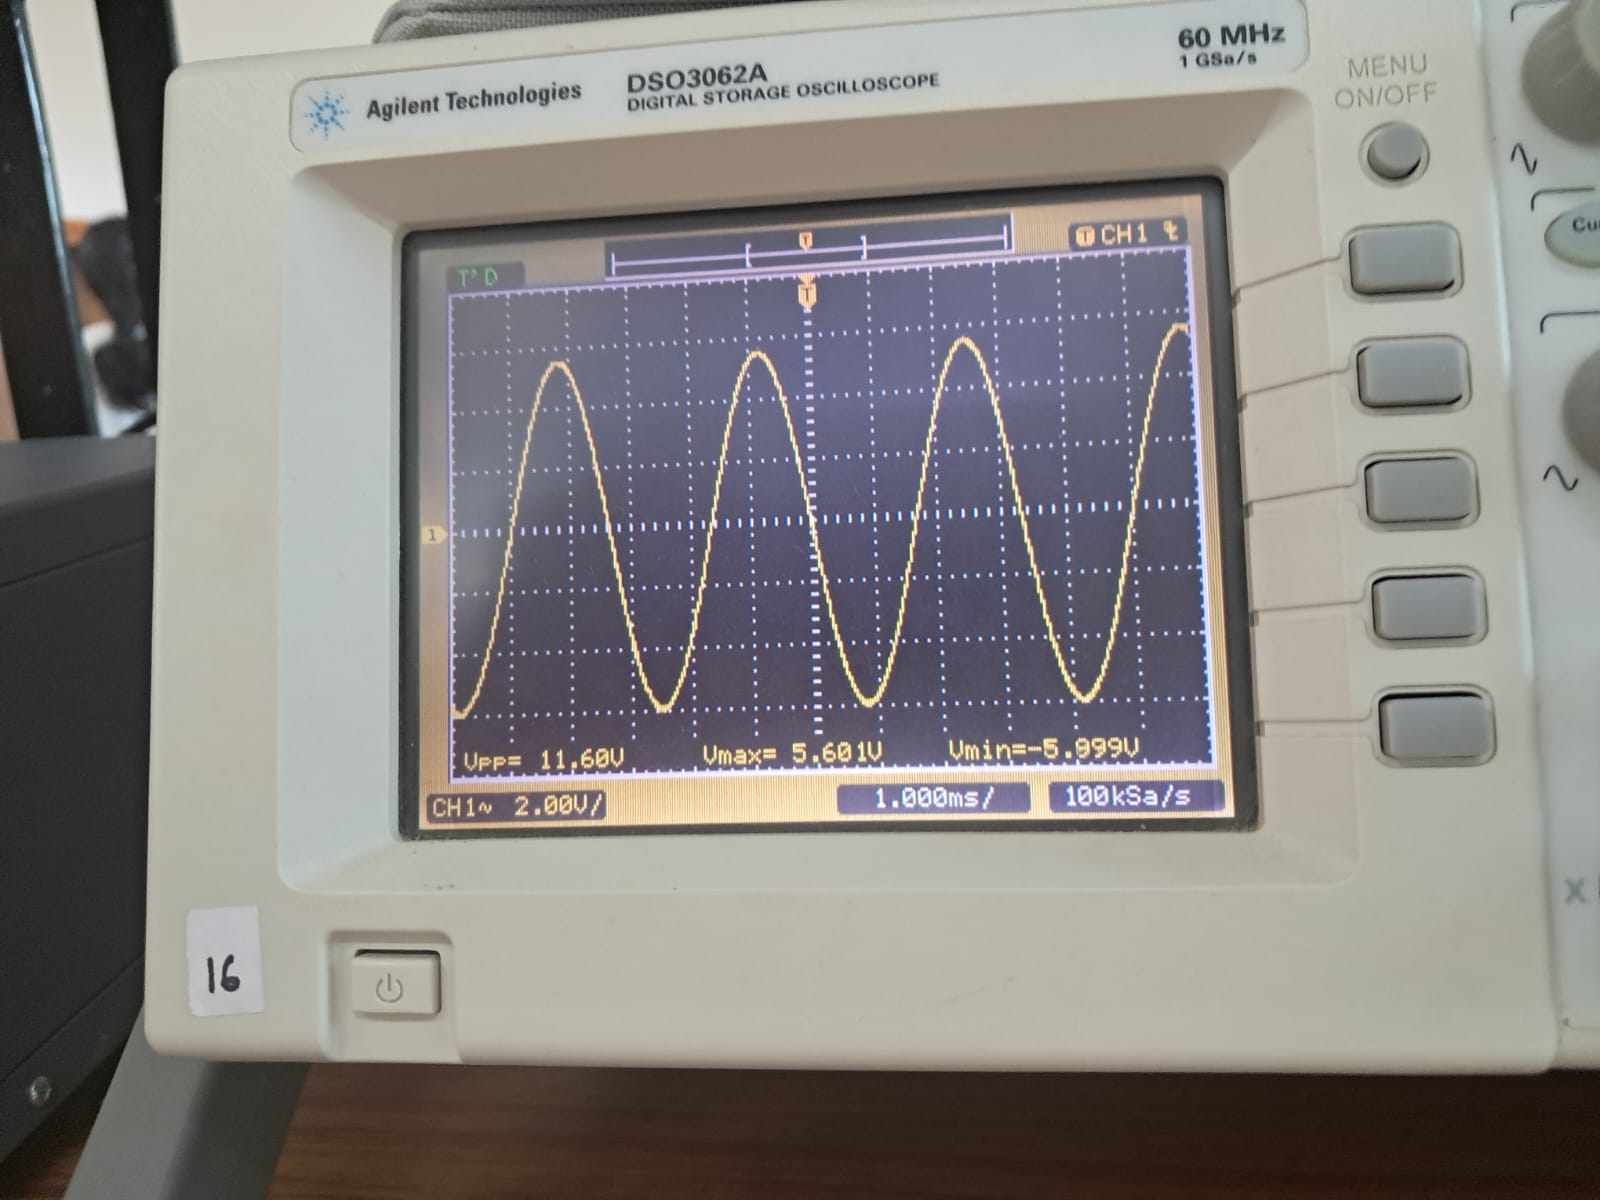
\includegraphics[width=\textwidth]{fig/lp/300o.jpeg}
        \caption{Oscilloscope reading for frequency 300Hz}
        %\label{fig:image1}
    \end{minipage}
    \hfill
    \begin{minipage}[b]{0.45\textwidth}
        \centering
        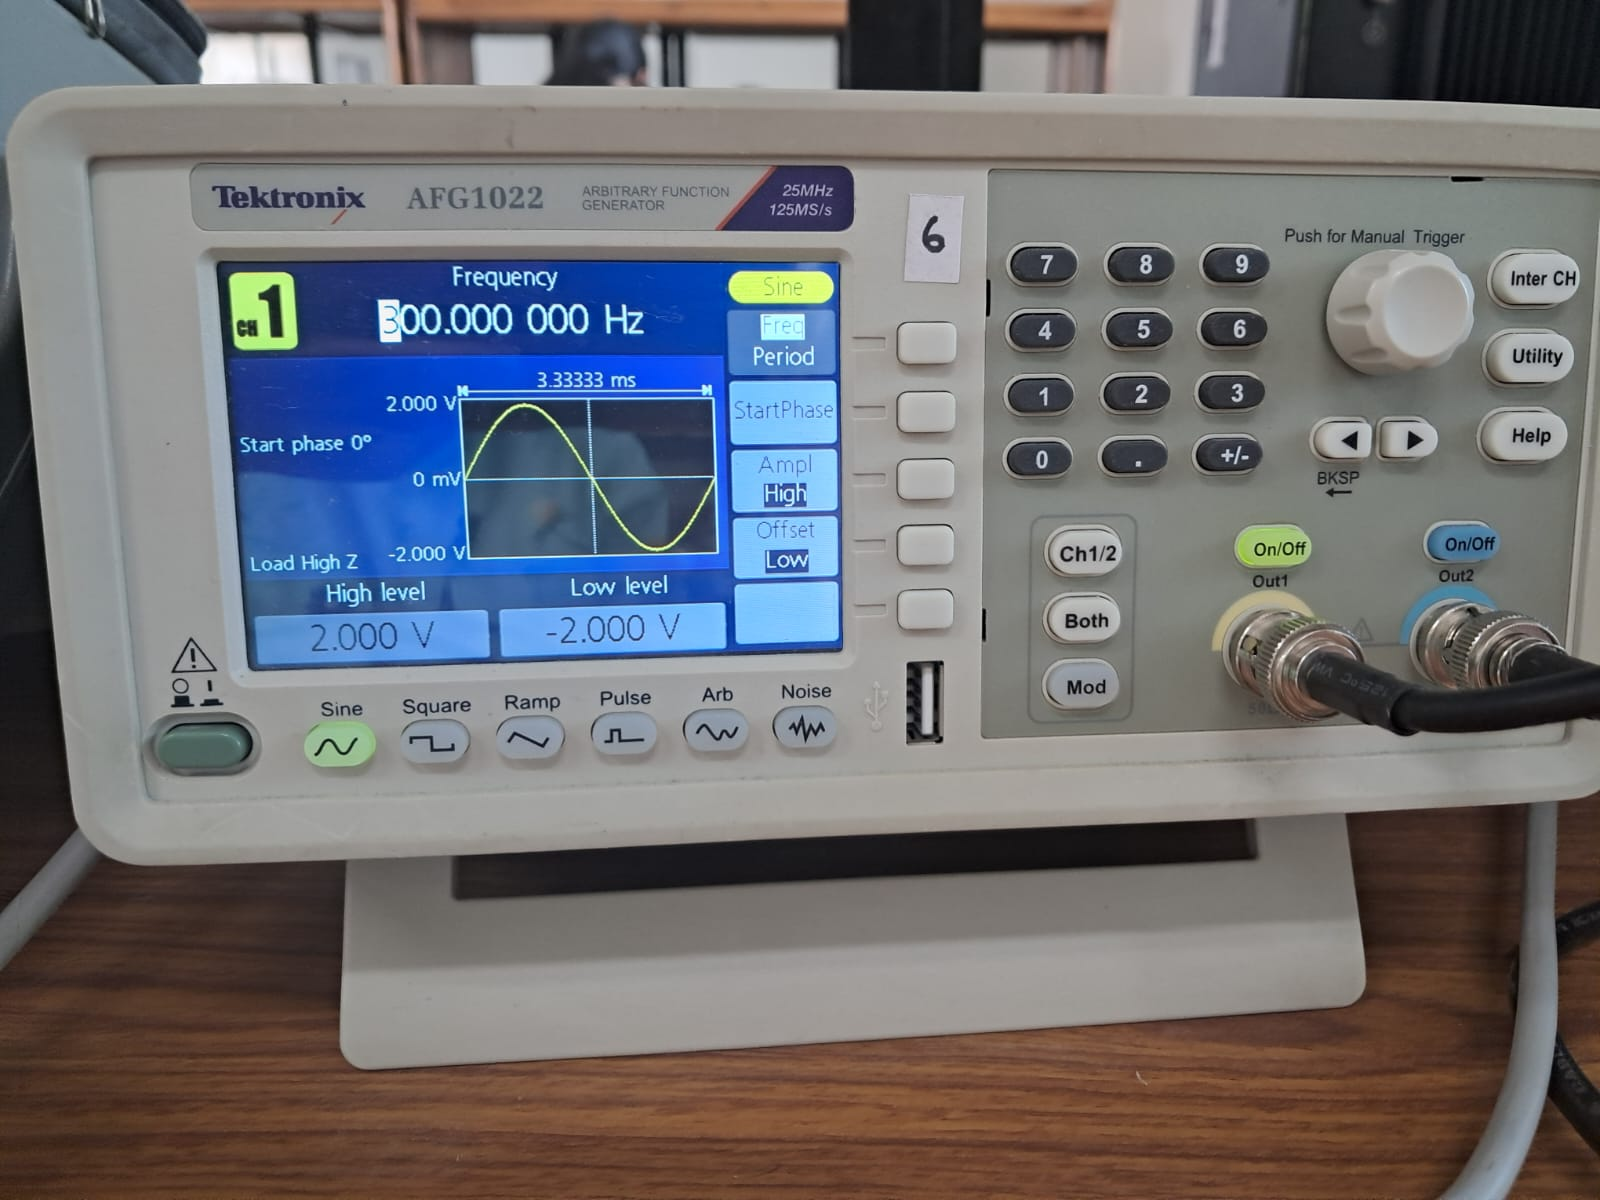
\includegraphics[width=\textwidth]{fig/lp/300.jpeg}
        \caption{FG}
        %\label{fig:image2}
    \end{minipage}
\end{figure}

\begin{figure}[H]
    \centering
    \begin{minipage}[b]{0.45\textwidth}
        \centering
        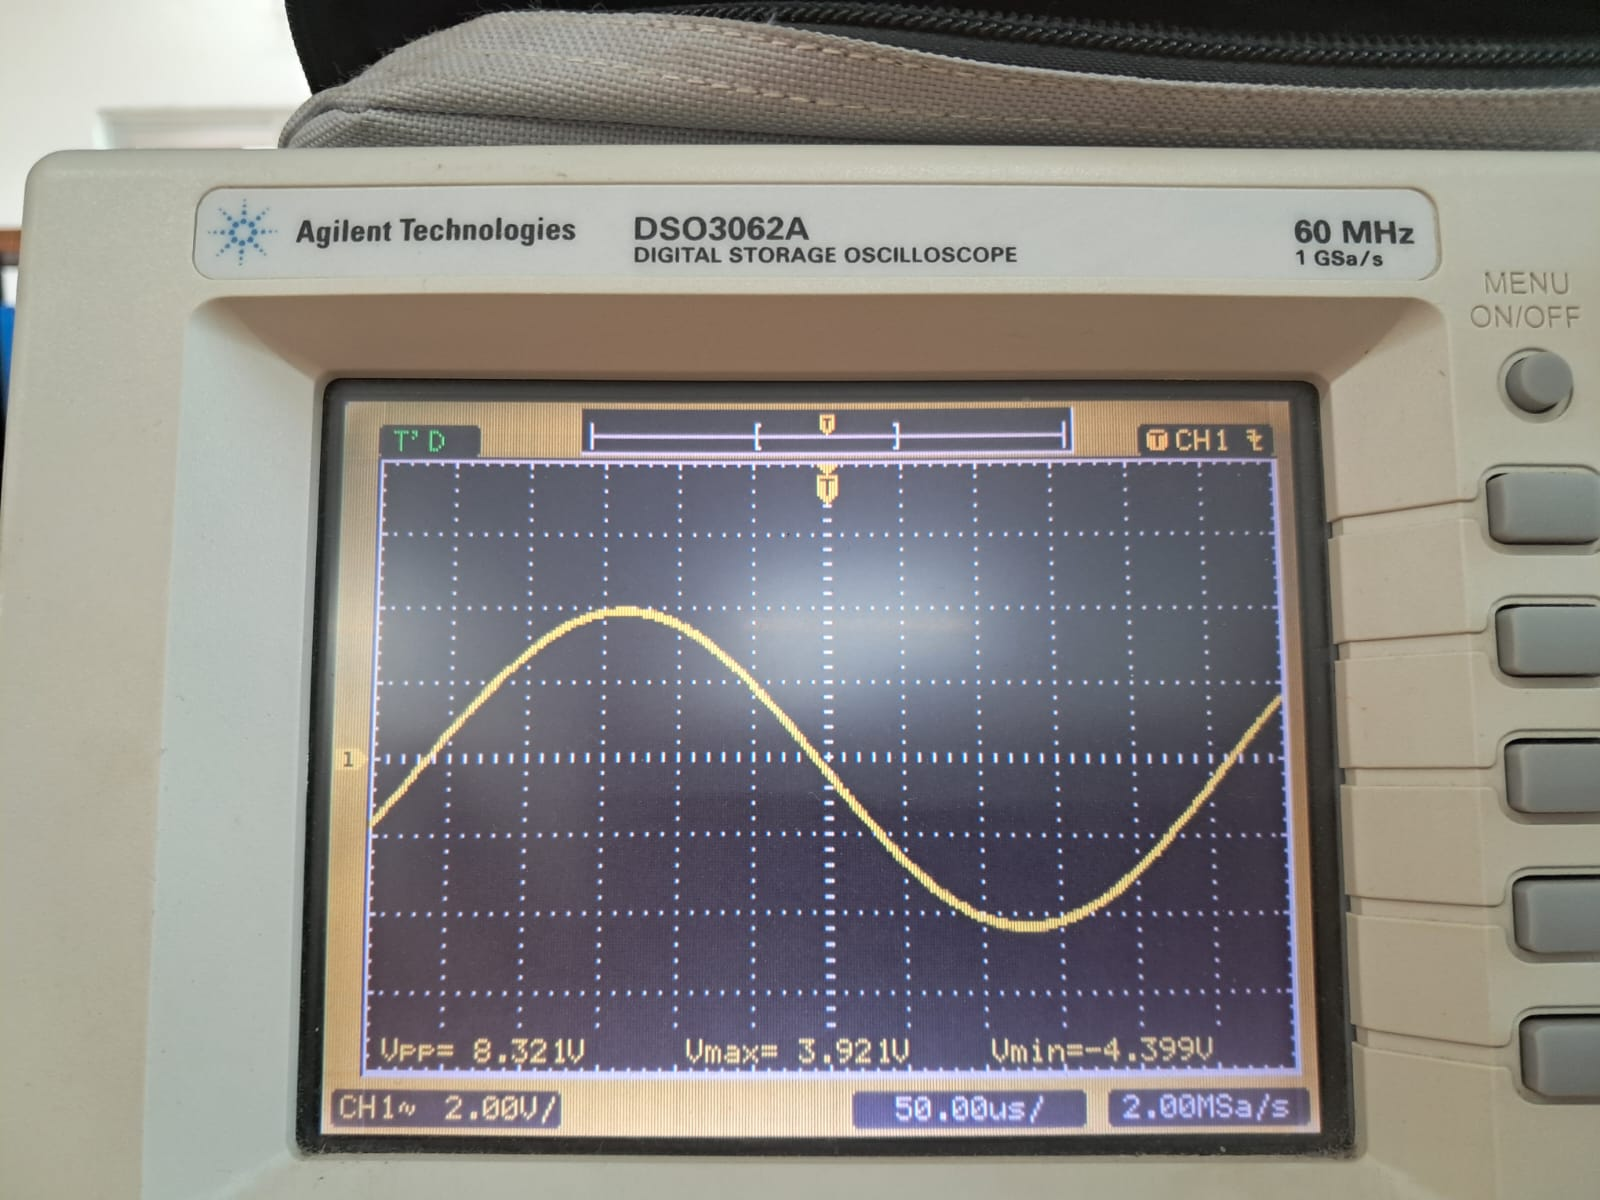
\includegraphics[width=\textwidth]{fig/lp/1.8ko.jpeg}
        \caption{Oscilloscope reading for frequency 1.8kHz}
        %\label{fig:image1}
    \end{minipage}
    \hfill
    \begin{minipage}[b]{0.45\textwidth}
        \centering
        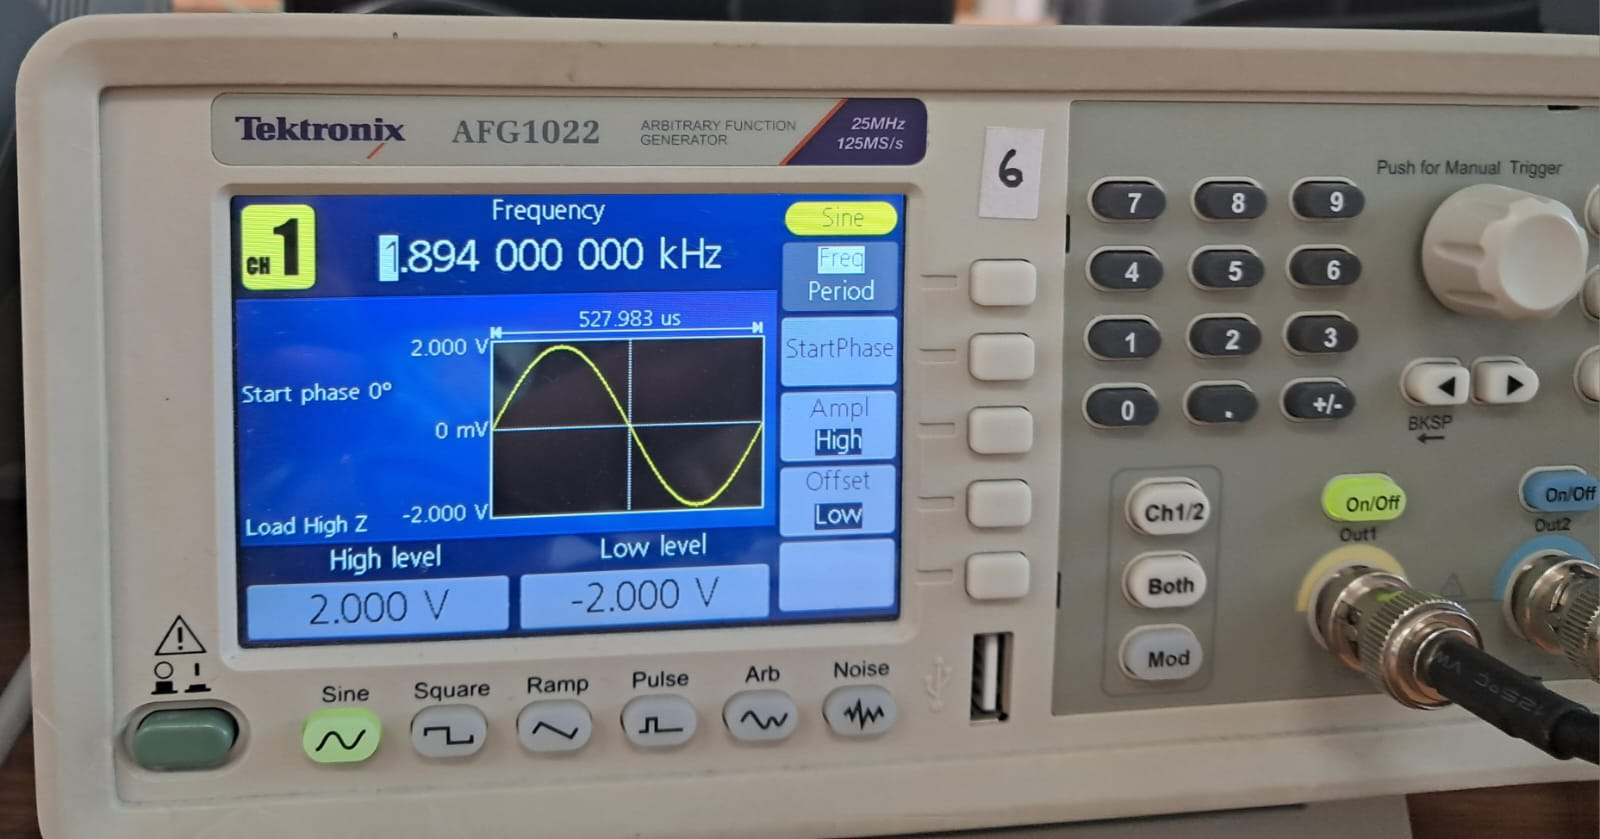
\includegraphics[width=\textwidth]{fig/lp/1.8k.jpeg}
        \caption{FG}
        %\label{fig:image2}
    \end{minipage}
\end{figure}

\begin{figure}[H]
    \centering
    \begin{minipage}[b]{0.45\textwidth}
        \centering
        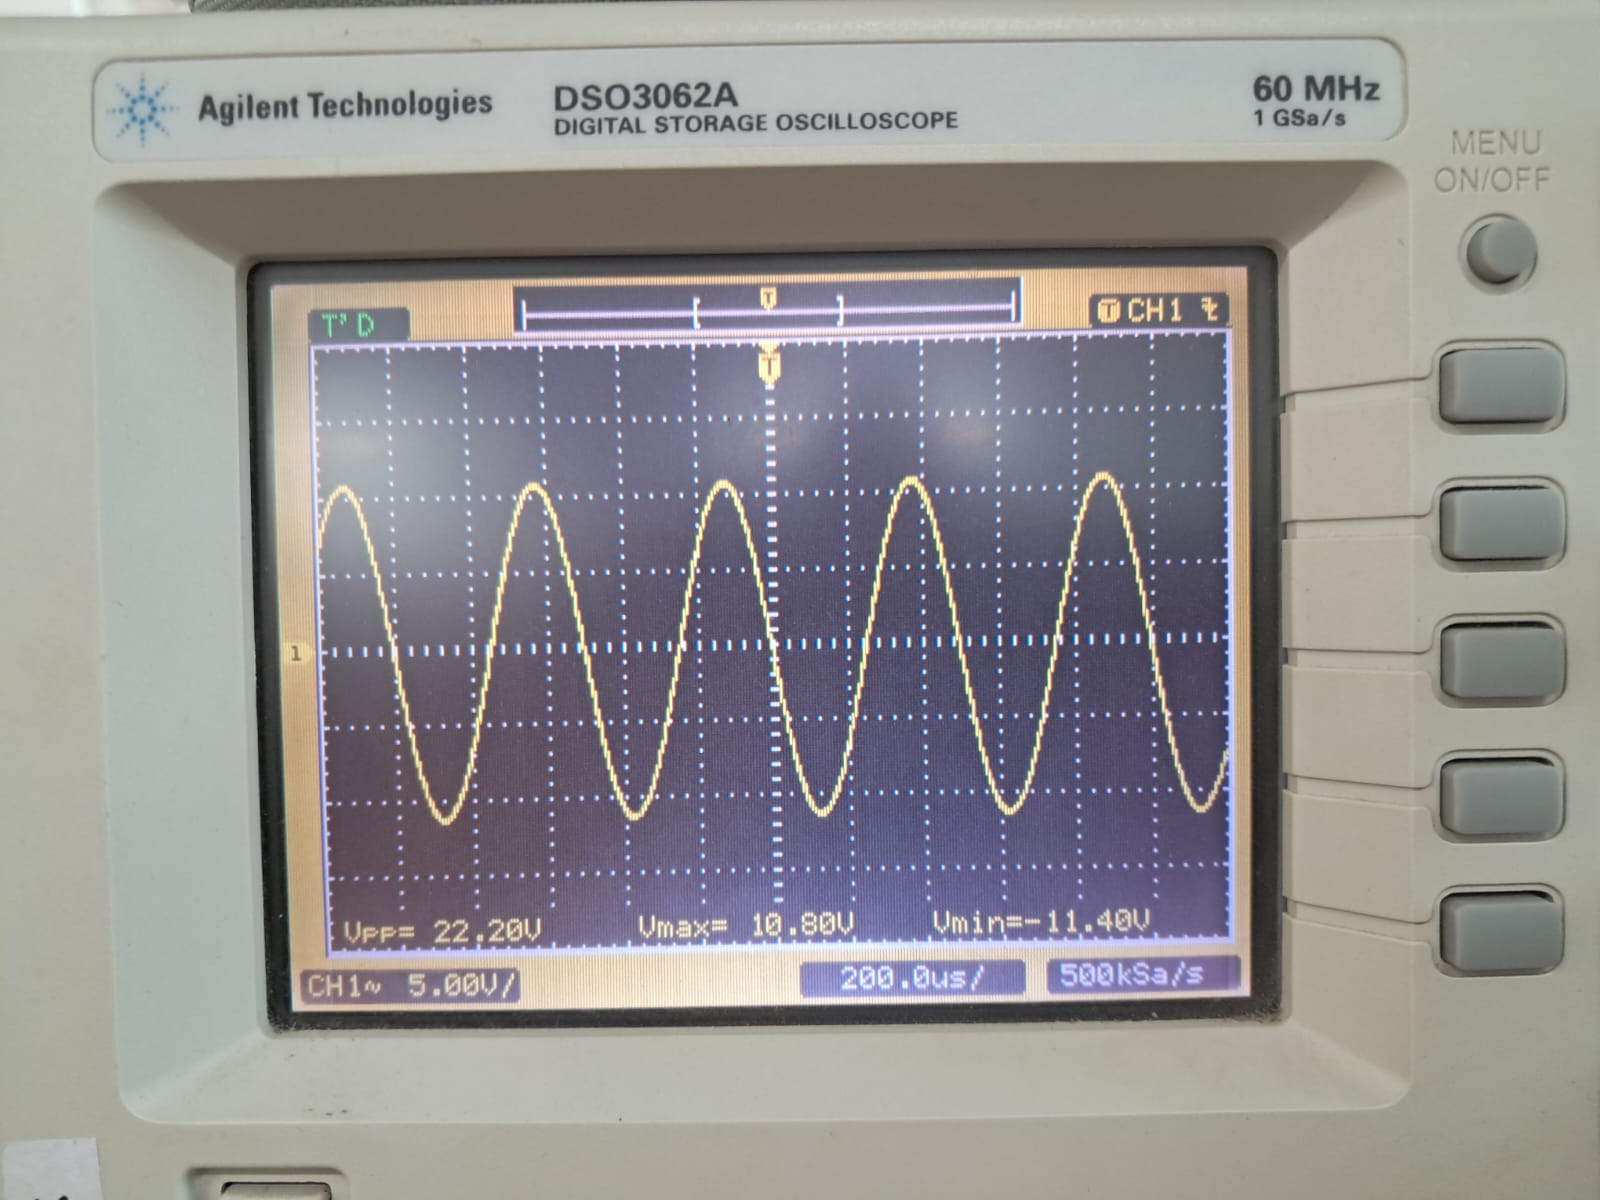
\includegraphics[width=\textwidth]{fig/lp/2ko.jpeg}
        \caption{Oscilloscope reading for frequency 2kHz}
        %\label{fig:image1}
    \end{minipage}
    \hfill
    \begin{minipage}[b]{0.45\textwidth}
        \centering
        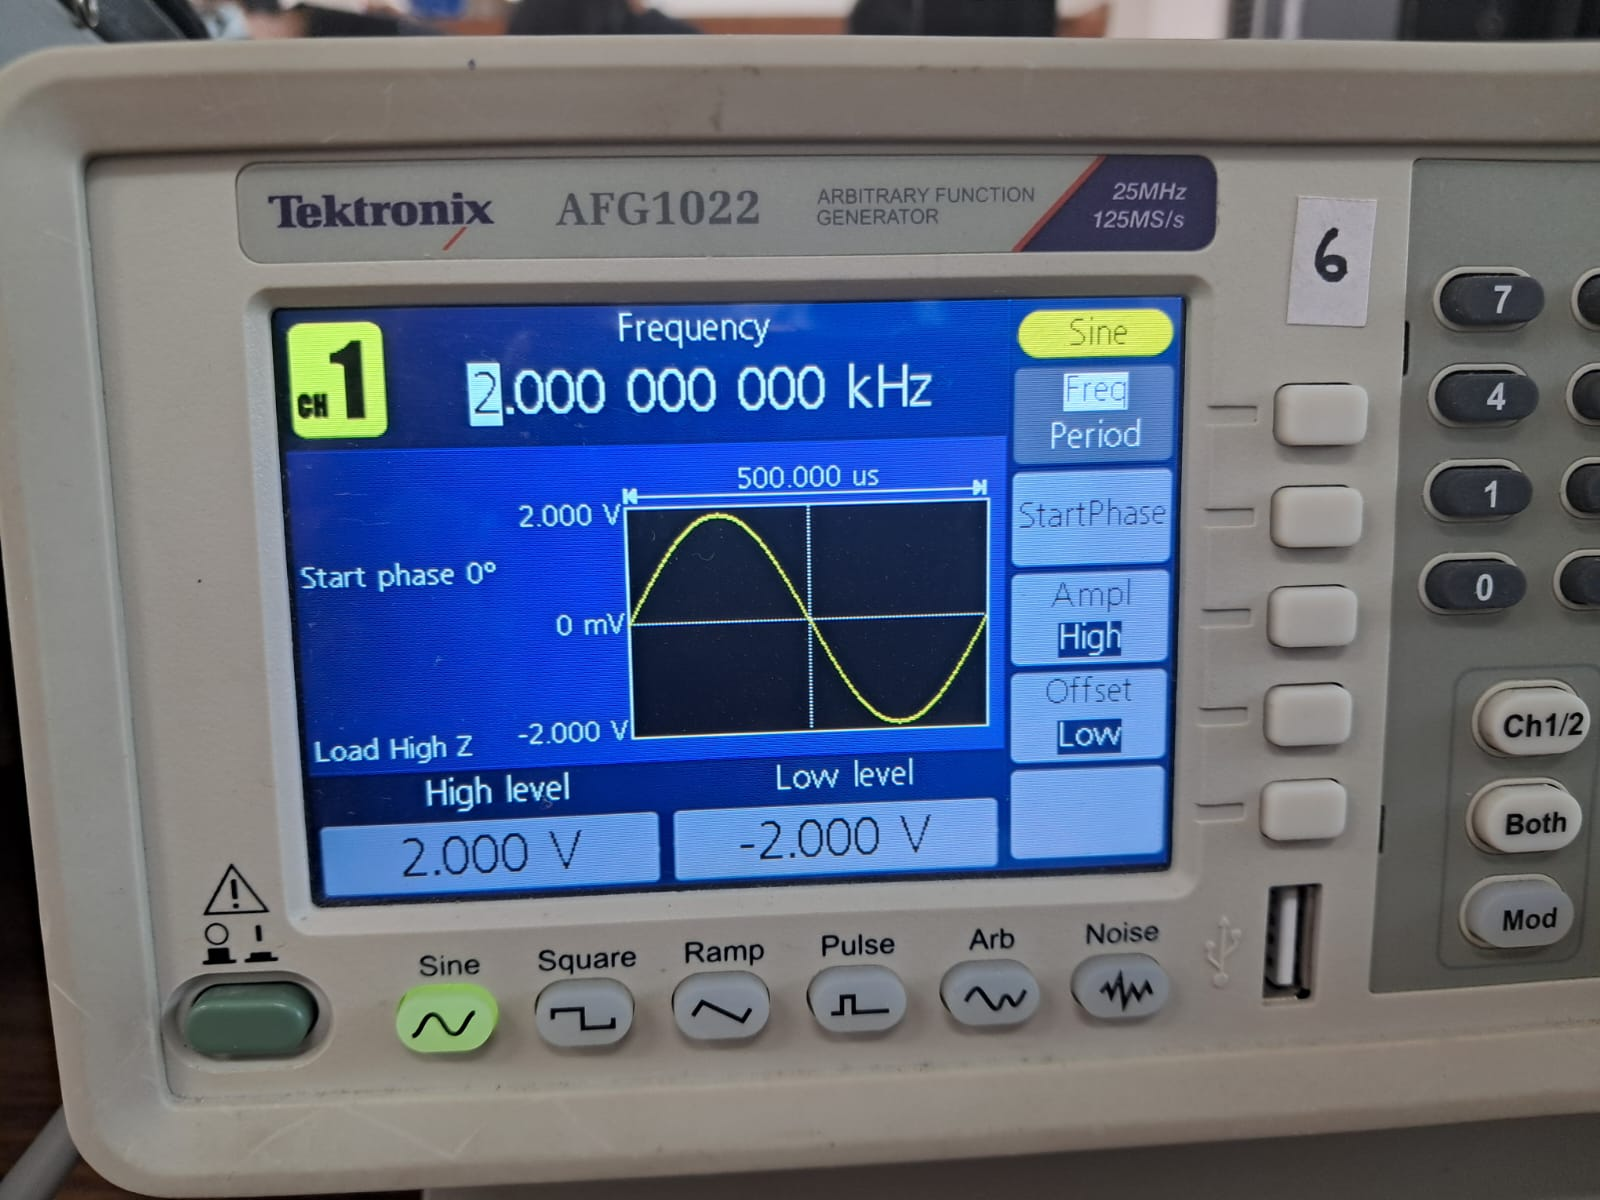
\includegraphics[width=\textwidth]{fig/lp/2k.jpeg}
        \caption{FG}
        %\label{fig:image2}
    \end{minipage}
\end{figure}

\begin{figure}[H]
    \centering
    \begin{minipage}[b]{0.45\textwidth}
        \centering
        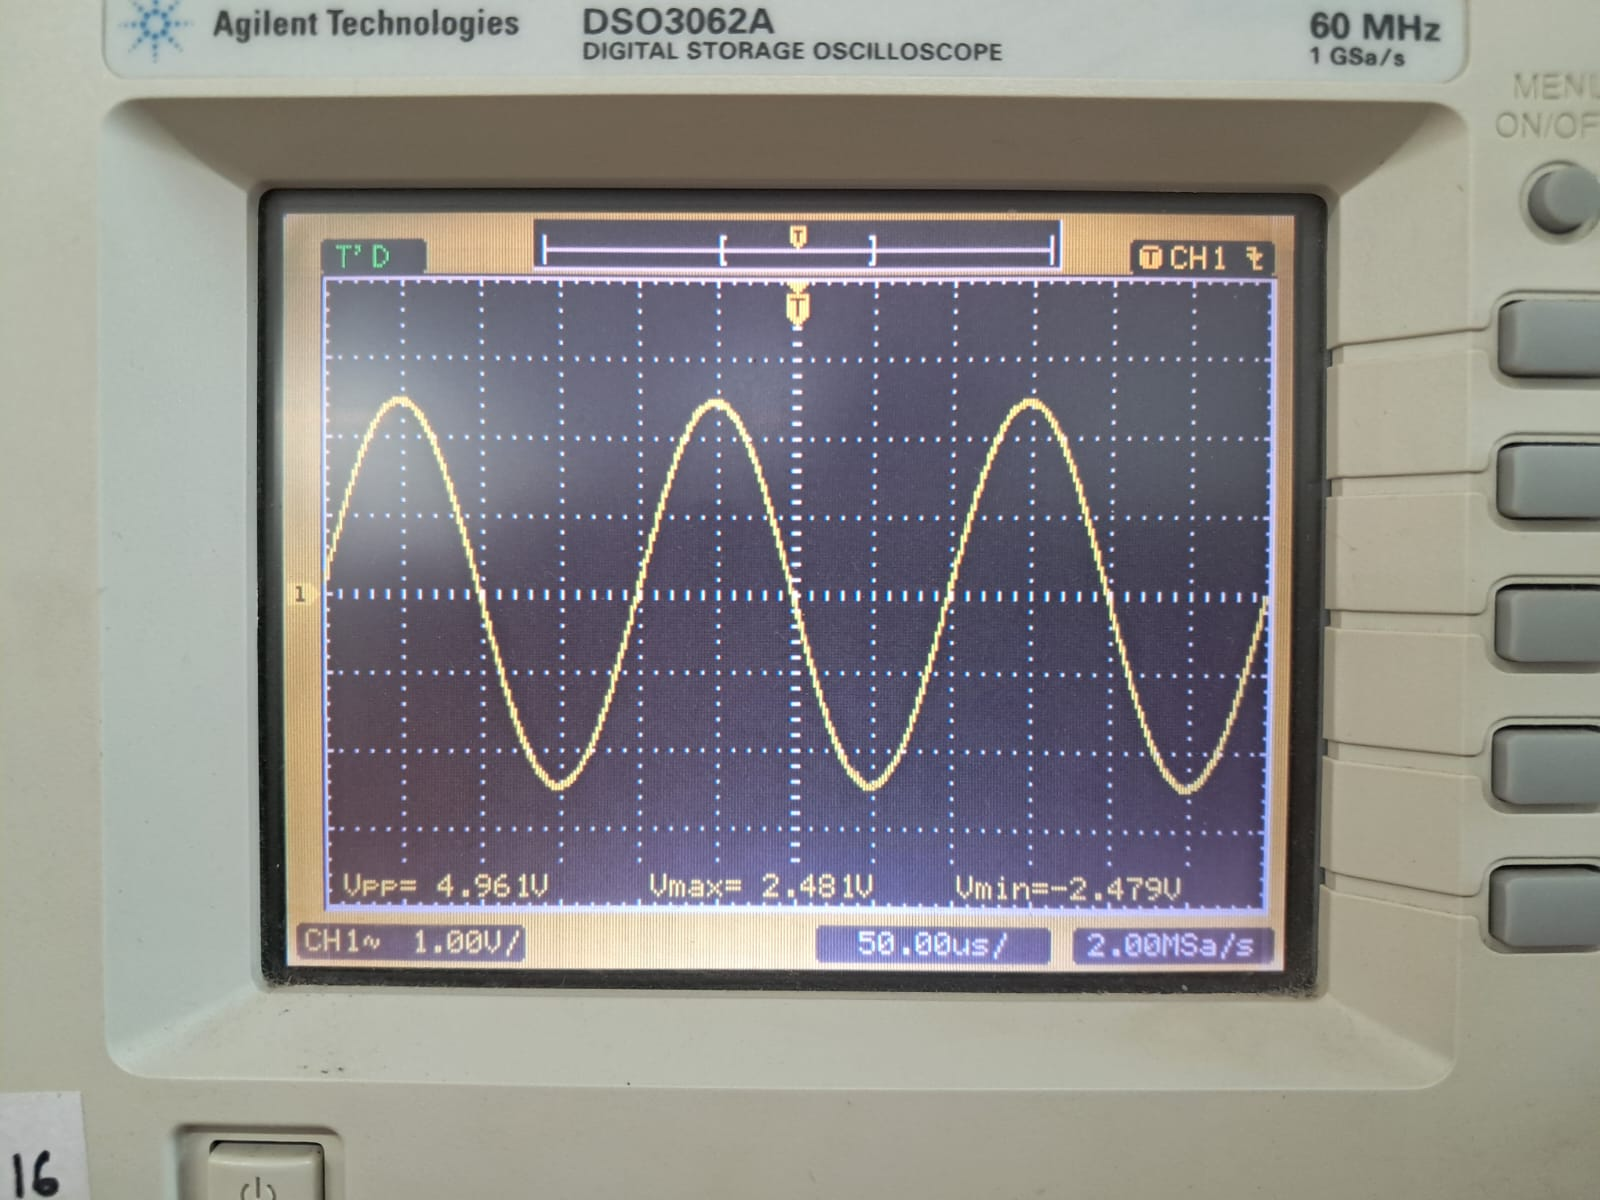
\includegraphics[width=\textwidth]{fig/lp/5ko.jpeg}
        \caption{Oscilloscope reading for frequency 5kHz}
        %\label{fig:image1}
    \end{minipage}
    \hfill
    \begin{minipage}[b]{0.45\textwidth}
        \centering
        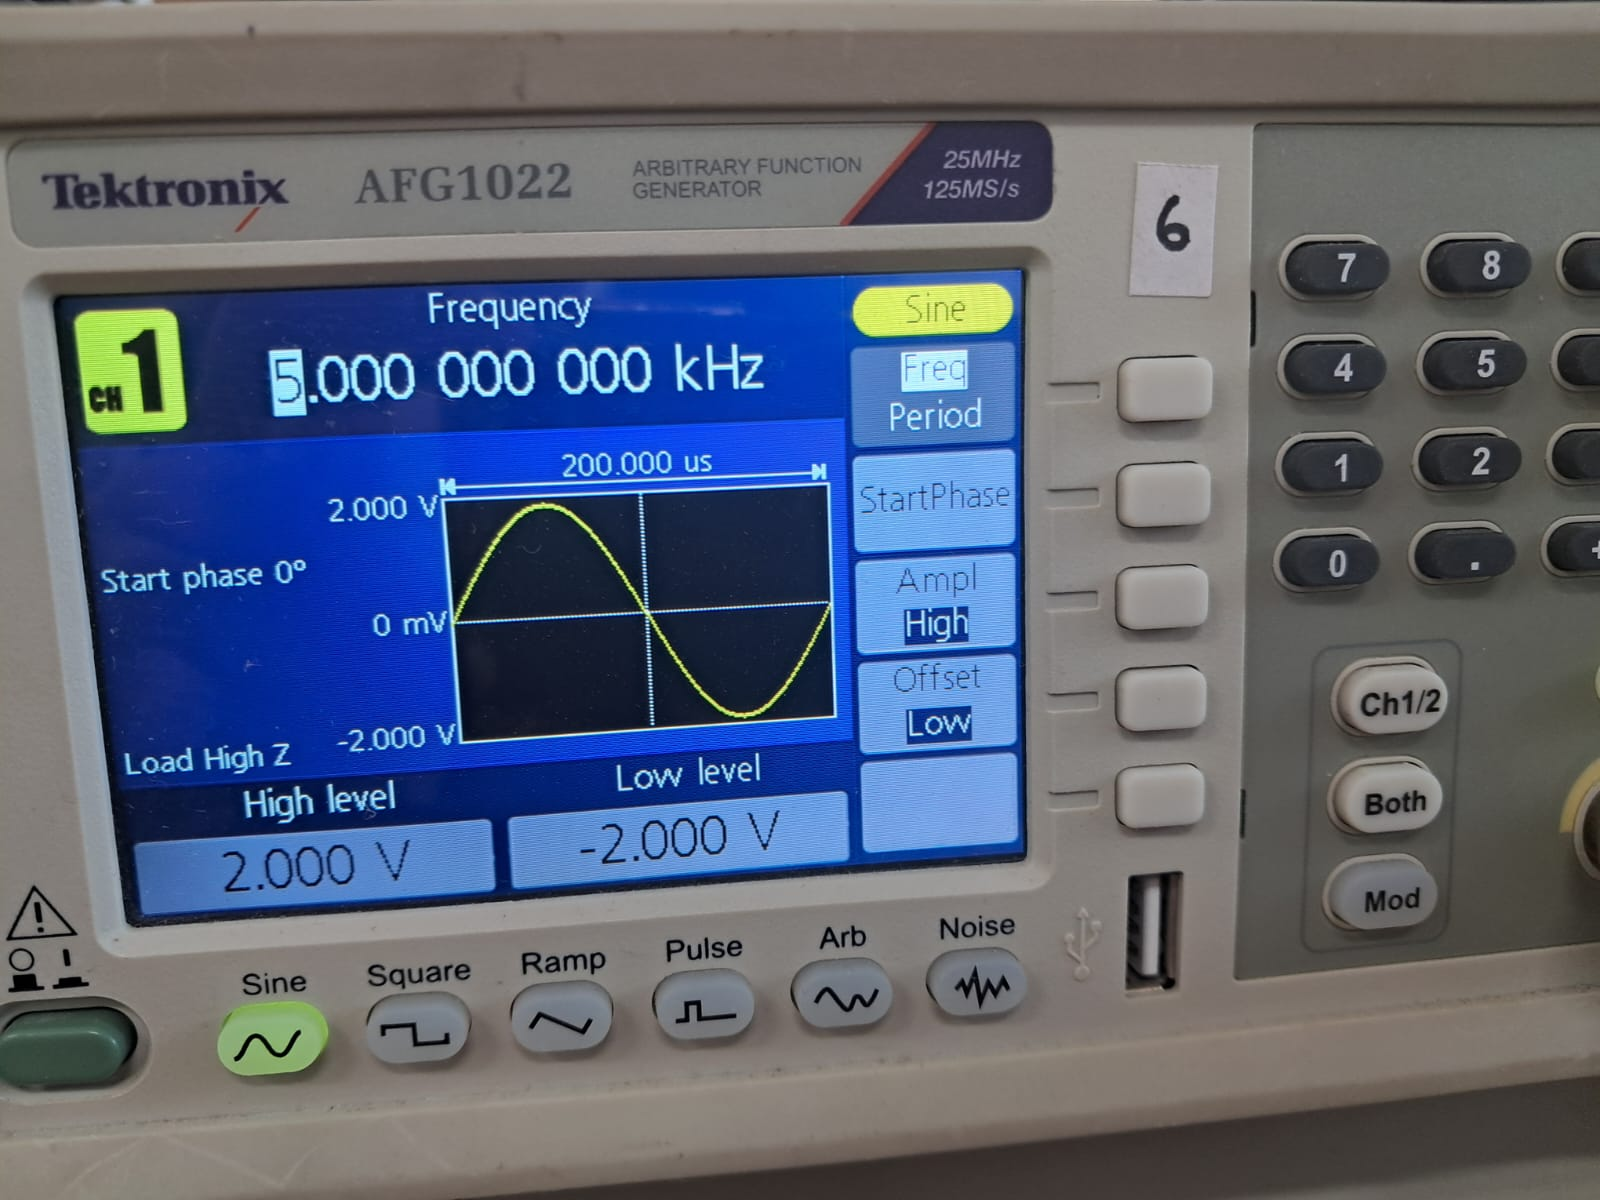
\includegraphics[width=\textwidth]{fig/lp/5k.jpeg}
        \caption{FG}
        %\label{fig:image2}
    \end{minipage}
\end{figure}
\subsubsection{Bode plot}

\begin{figure}[H]
    \centering
    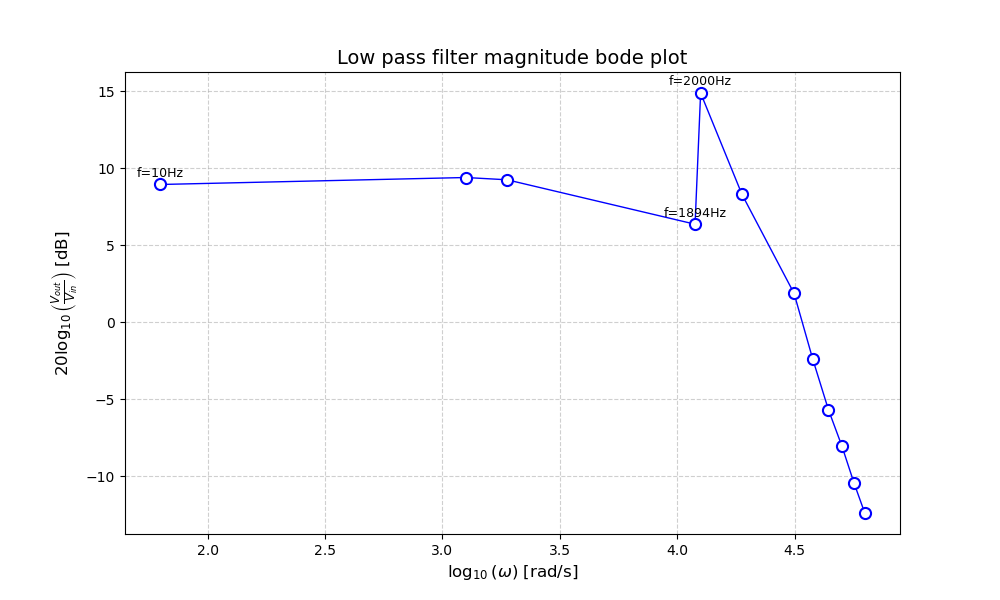
\includegraphics[width=0.8\textwidth]{fig/lpb.png}
    \caption{Low pass BP- Measured}
    \label{fig:your-label}
\end{figure}

\begin{figure}[H]
    \centering
    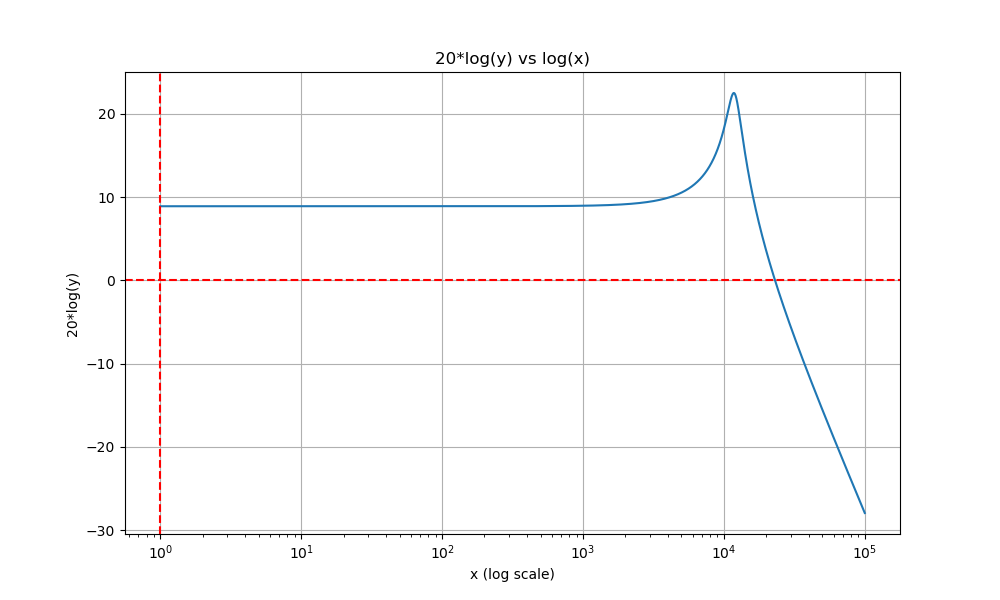
\includegraphics[width=0.8\textwidth]{lpfp.png}
    \caption{Low pass BP- Theoretical}
    \label{fig:your-label}
\end{figure}


\subsection{High-Pass Filter}
\begin{enumerate}
     \item Assemble the Sallen-key HPF circuit on the breadboard.
    \item Use the function Generator to apply a sine wave.
    \item Vary the input frequency and measure the output voltage.
    \item Record gain values for different frequencies.
    \item Plot gain vs. frequency (Bode plot).
\end{enumerate}

\begin{figure}[H]
    \centering
    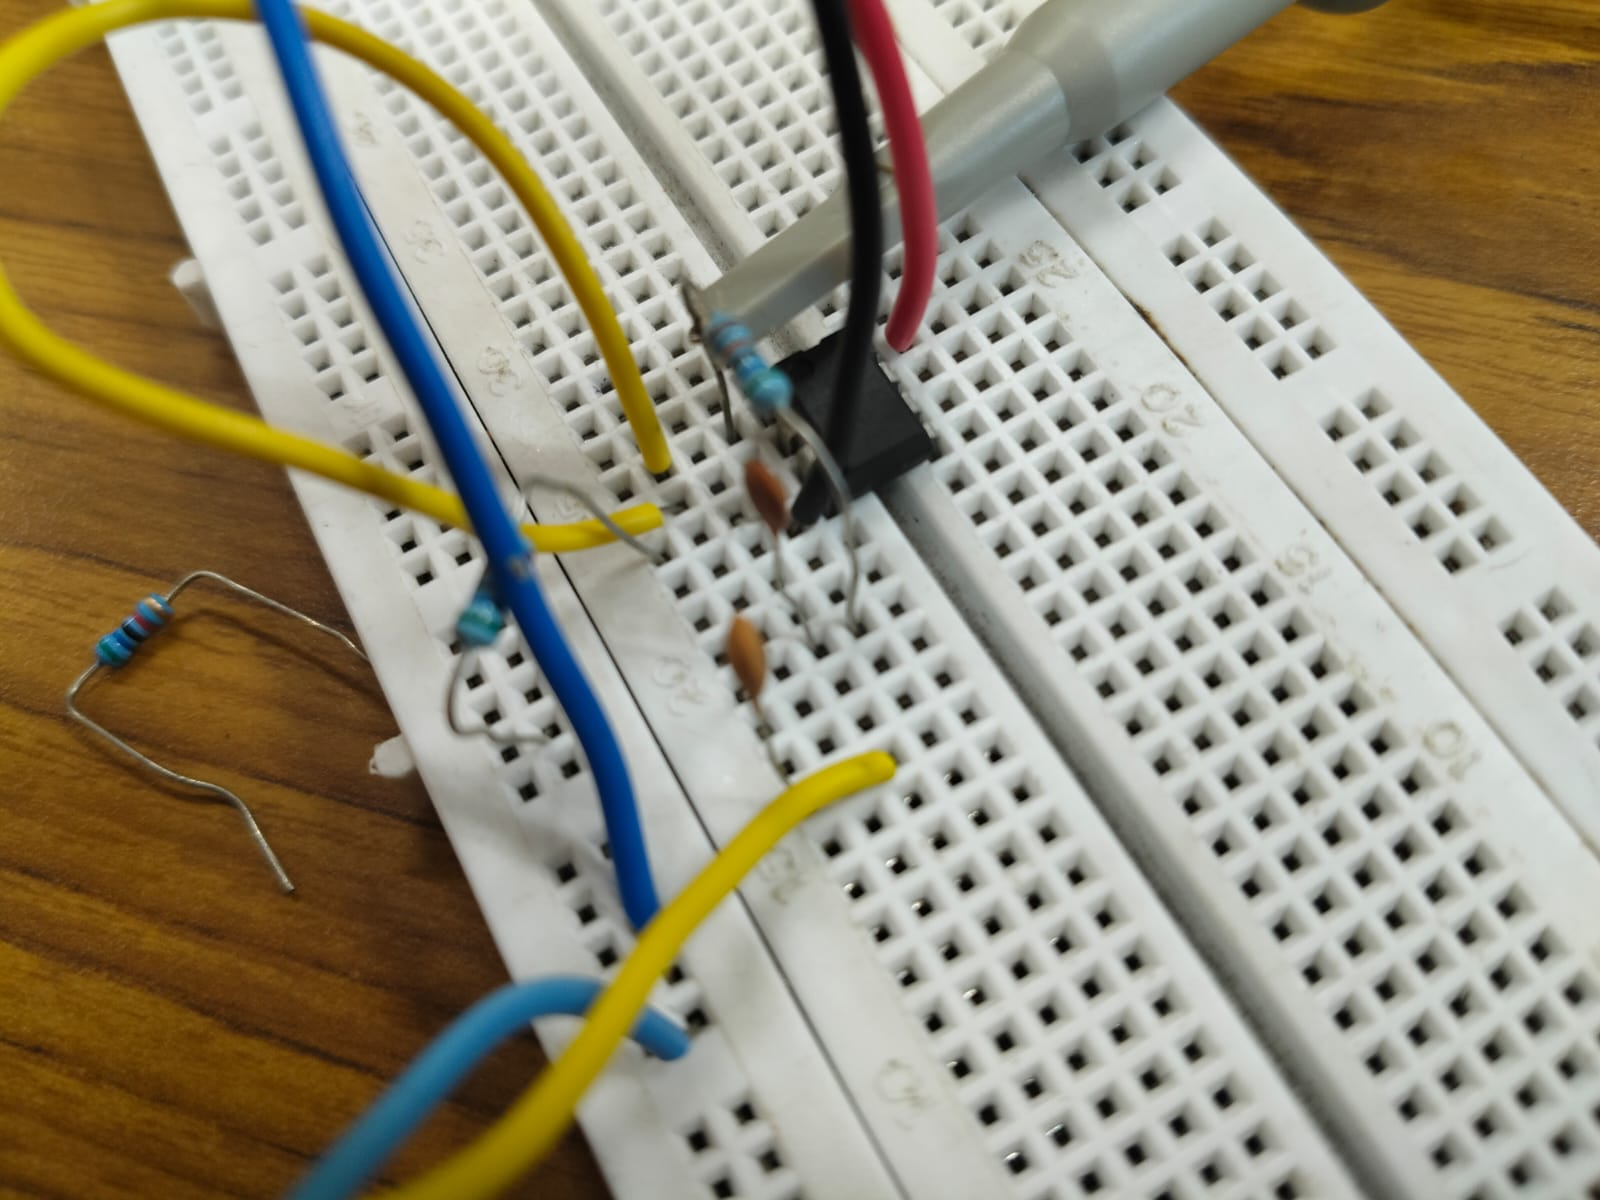
\includegraphics[width=0.8\textwidth]{fig/hp.jpeg}
    \caption{Circuit Diagram}
    \label{fig:your-label}
\end{figure}

\subsubsection{Observations}

\begin{figure}[H]
    \centering
    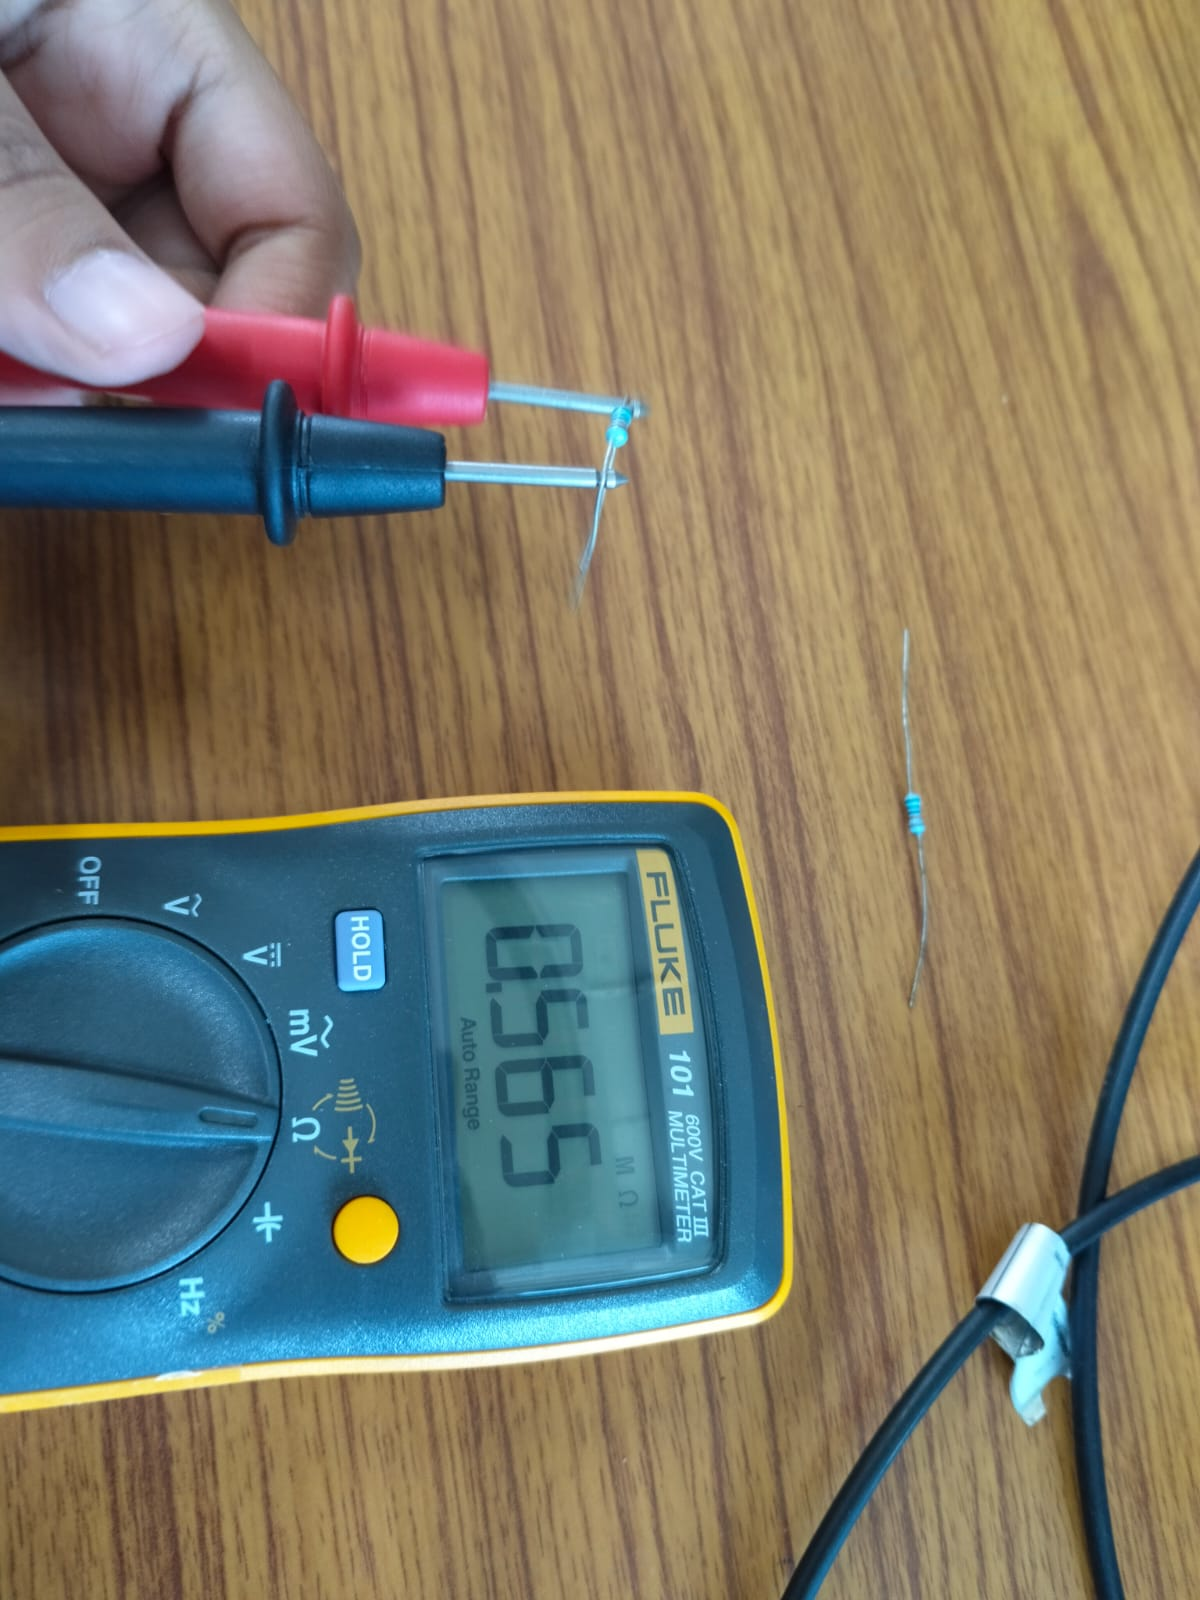
\includegraphics[width=0.8\textwidth]{fig/m/560kohm.jpeg}
    \caption{Resistance}
    \label{fig:your-label}
\end{figure}

\begin{table}[H]
\centering
\begin{tabular}{|c|c|c|}
\hline
\textbf{Frequency(in Hz)} & \textbf{Measured Values}  \\
\hline
500 & 1.001   \\
900 & 1.201    \\
7000 &   4.001   \\
10000 & 4.201   \\
11904 & 4.201  \\
20000 & 4.601   \\
50000 & 4.401  \\

\hline
\end{tabular}
\caption{Measured vs Theoretical Values}
\end{table}

\begin{figure}[H]
    \centering
    \begin{minipage}[b]{0.45\textwidth}
        \centering
        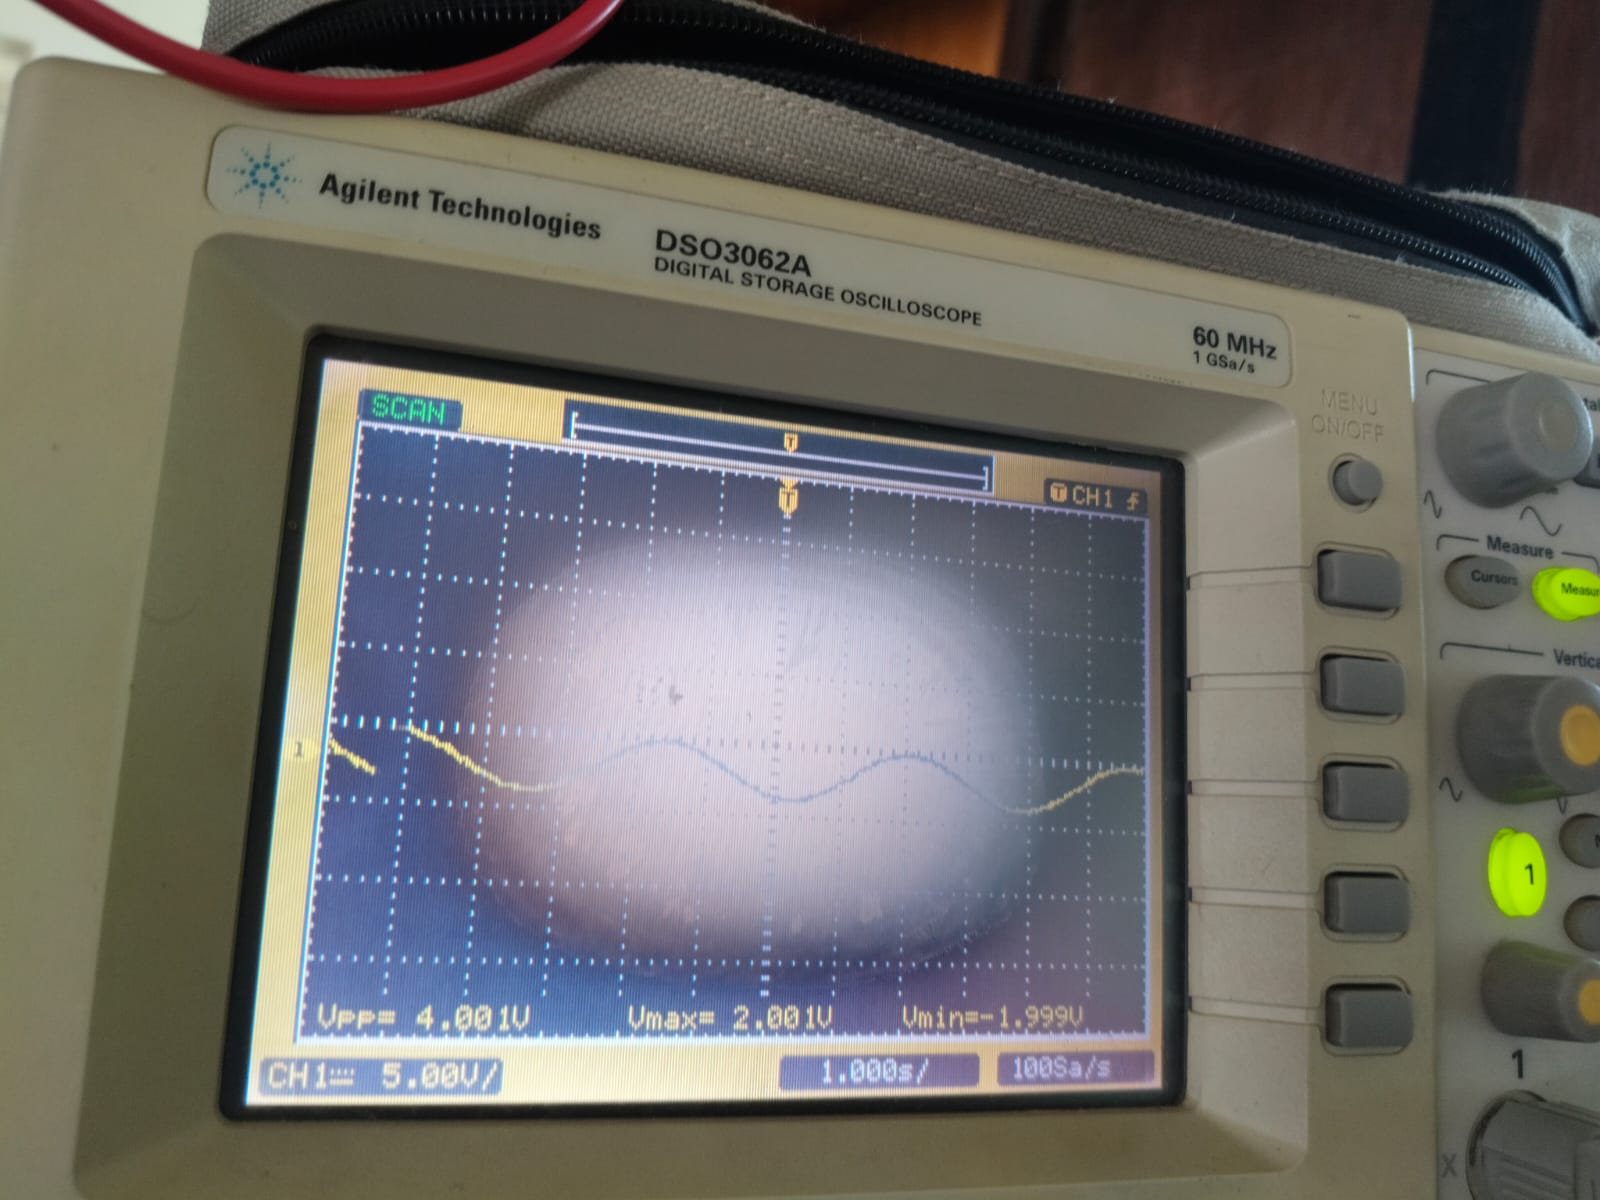
\includegraphics[width=\textwidth]{fig/hp/7ko.jpeg}
        \caption{Oscilloscope reading for frequency 7kHz}
        %\label{fig:image1}
    \end{minipage}
    \hfill
    \begin{minipage}[b]{0.45\textwidth}
        \centering
        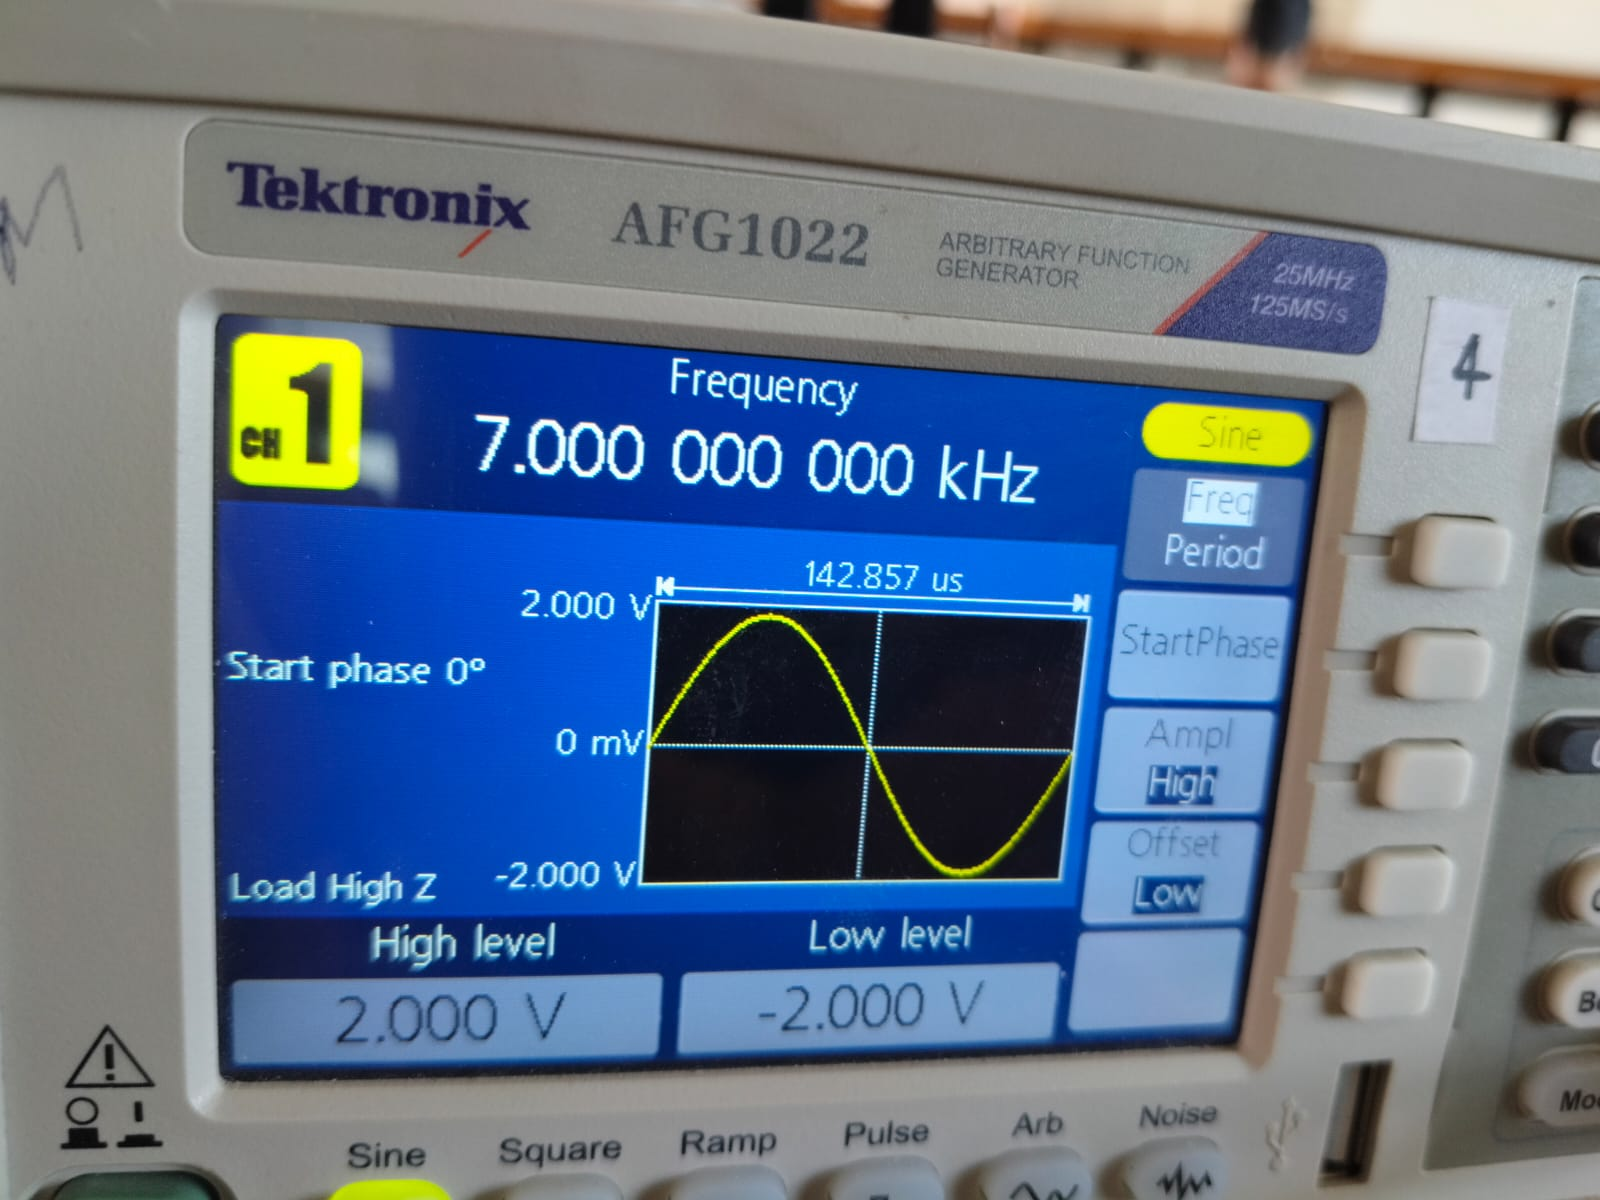
\includegraphics[width=\textwidth]{fig/hp/7k.jpeg}
        \caption{FG}
        %\label{fig:image2}
    \end{minipage}
\end{figure}

\begin{figure}[H]
    \centering
    \begin{minipage}[b]{0.45\textwidth}
        \centering
        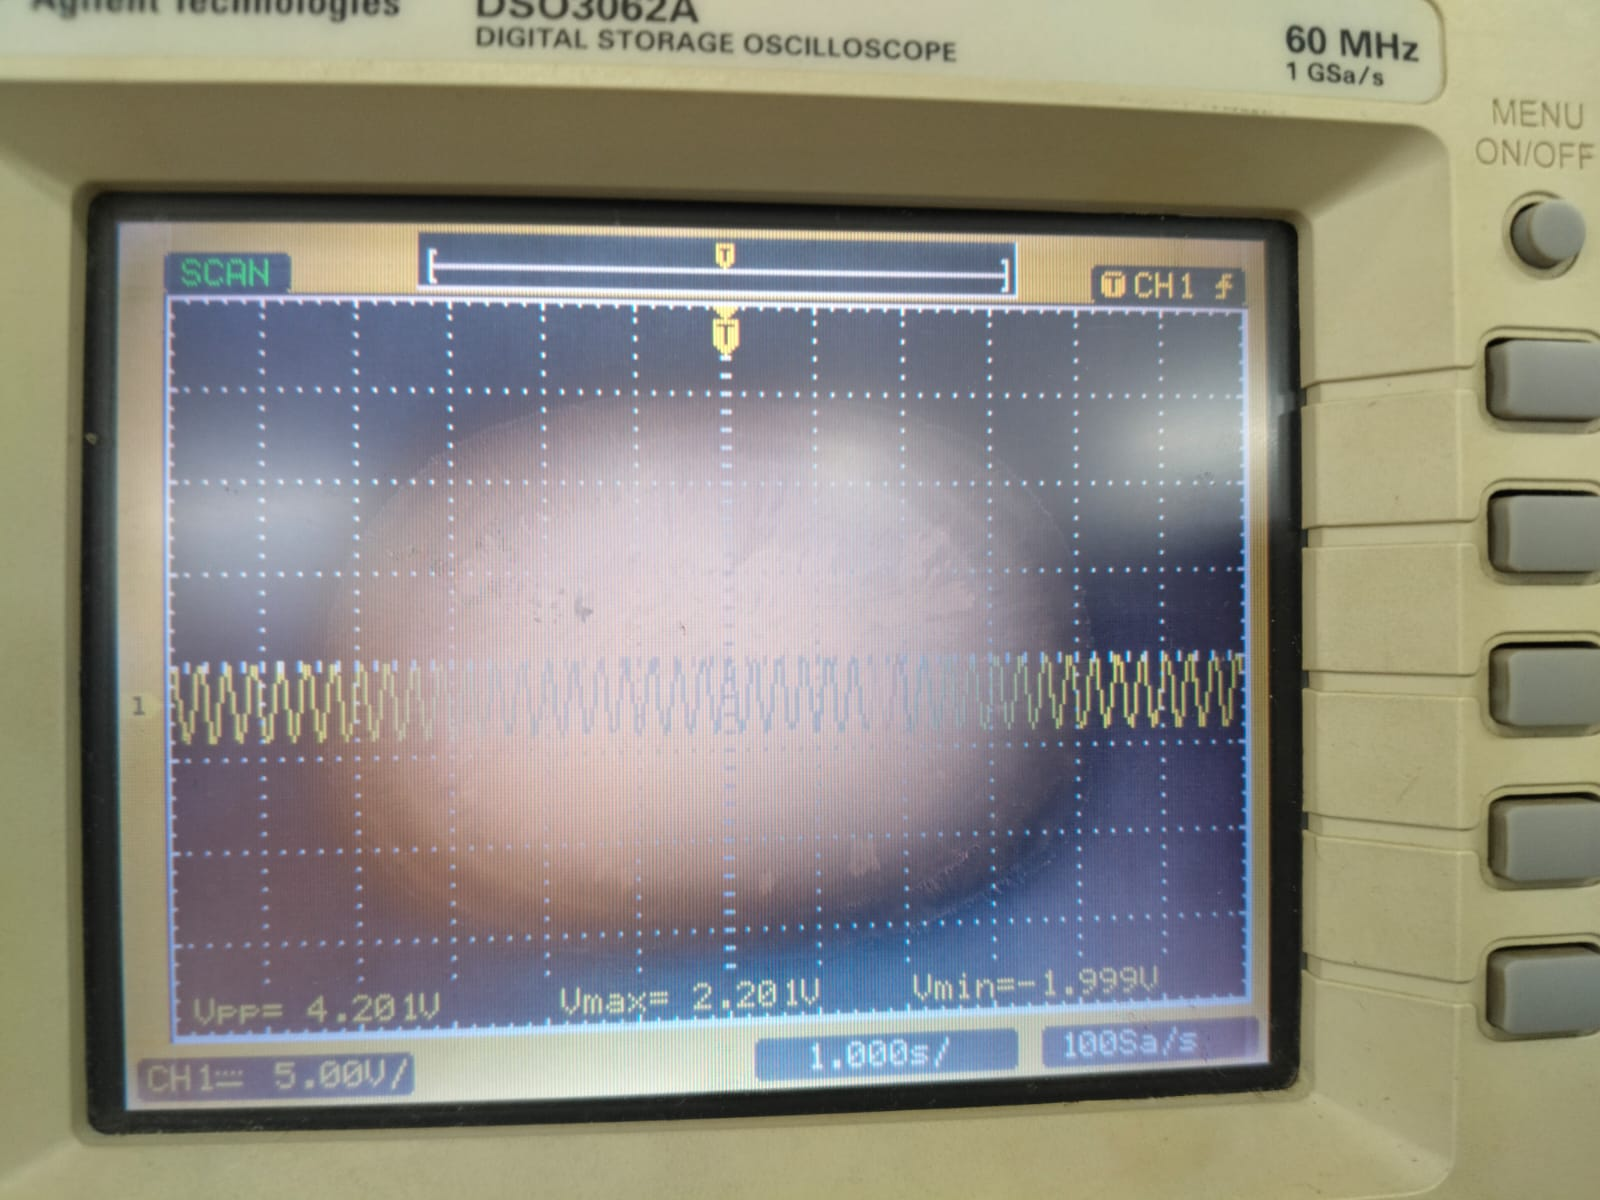
\includegraphics[width=\textwidth]{fig/hp/11ko.jpeg}
        \caption{Oscilloscope reading for frequency 11.904kHz}
        %\label{fig:image1}
    \end{minipage}
    \hfill
    \begin{minipage}[b]{0.45\textwidth}
        \centering
        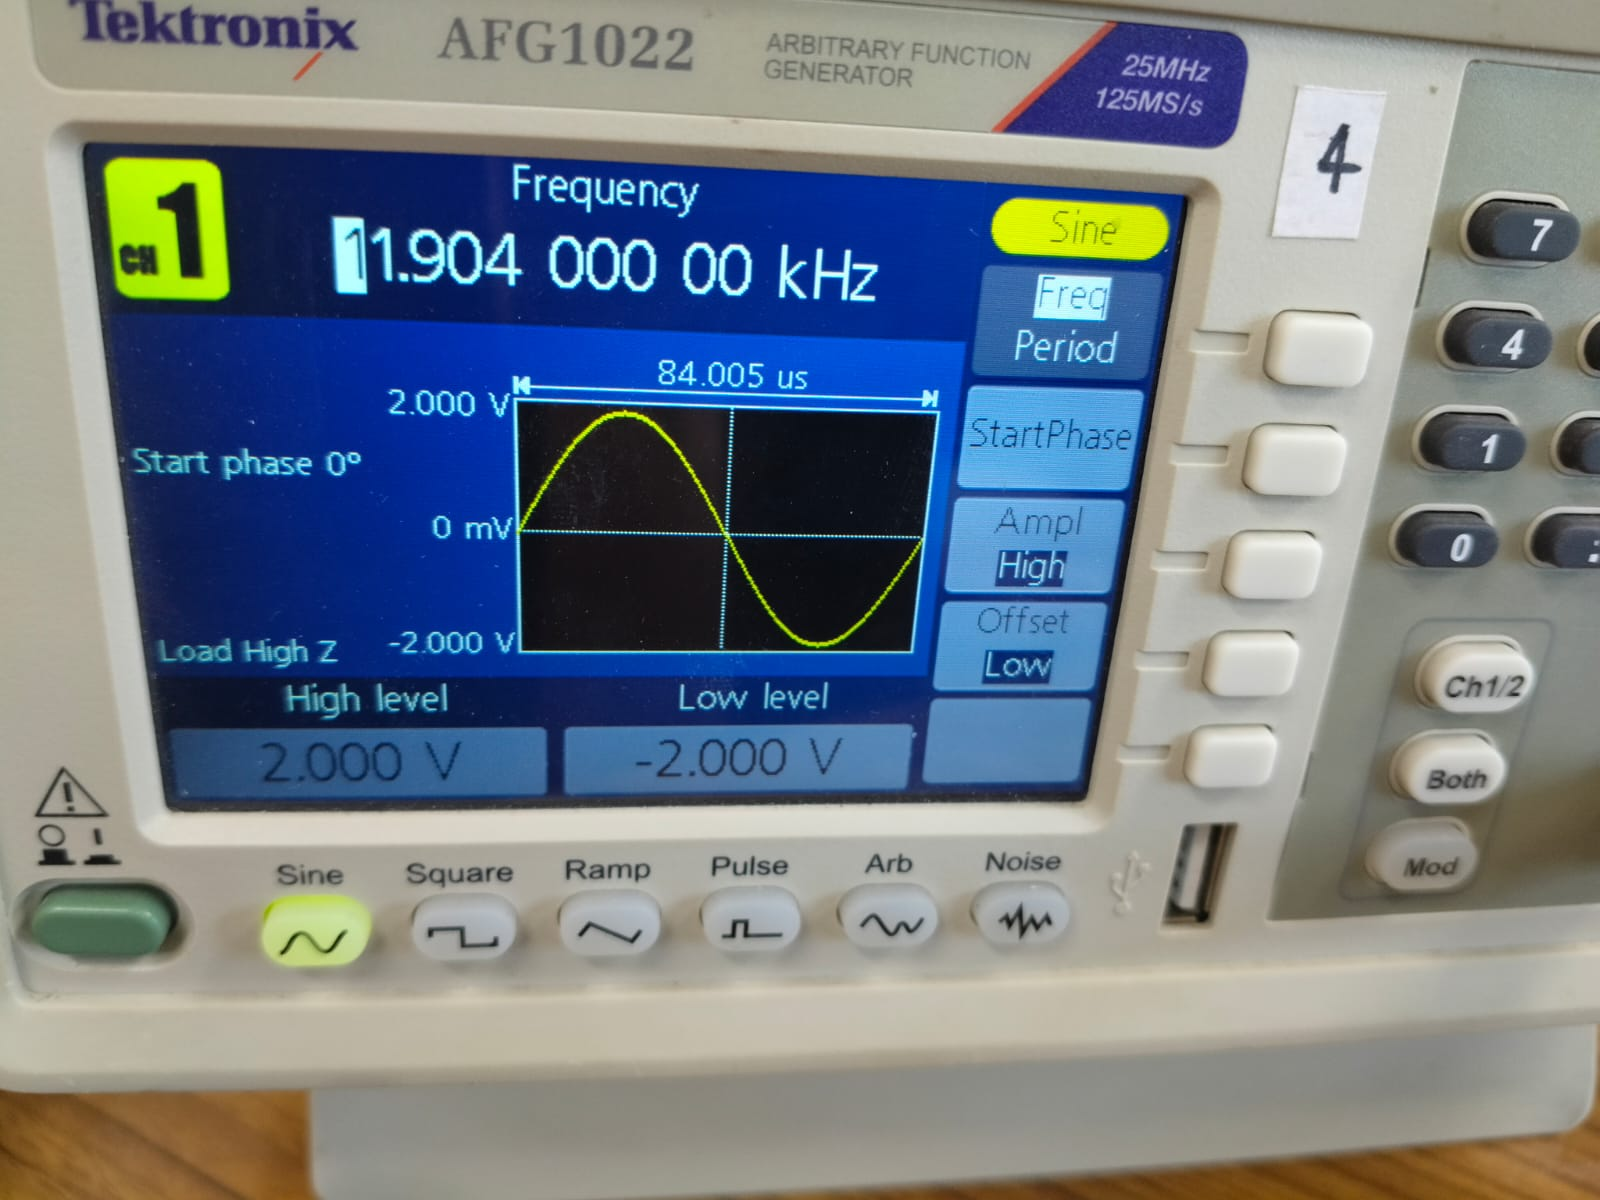
\includegraphics[width=\textwidth]{fig/hp/11k.jpeg}
        \caption{FG}
        %\label{fig:image2}
    \end{minipage}
\end{figure}

\begin{figure}[H]
    \centering
    \begin{minipage}[b]{0.45\textwidth}
        \centering
        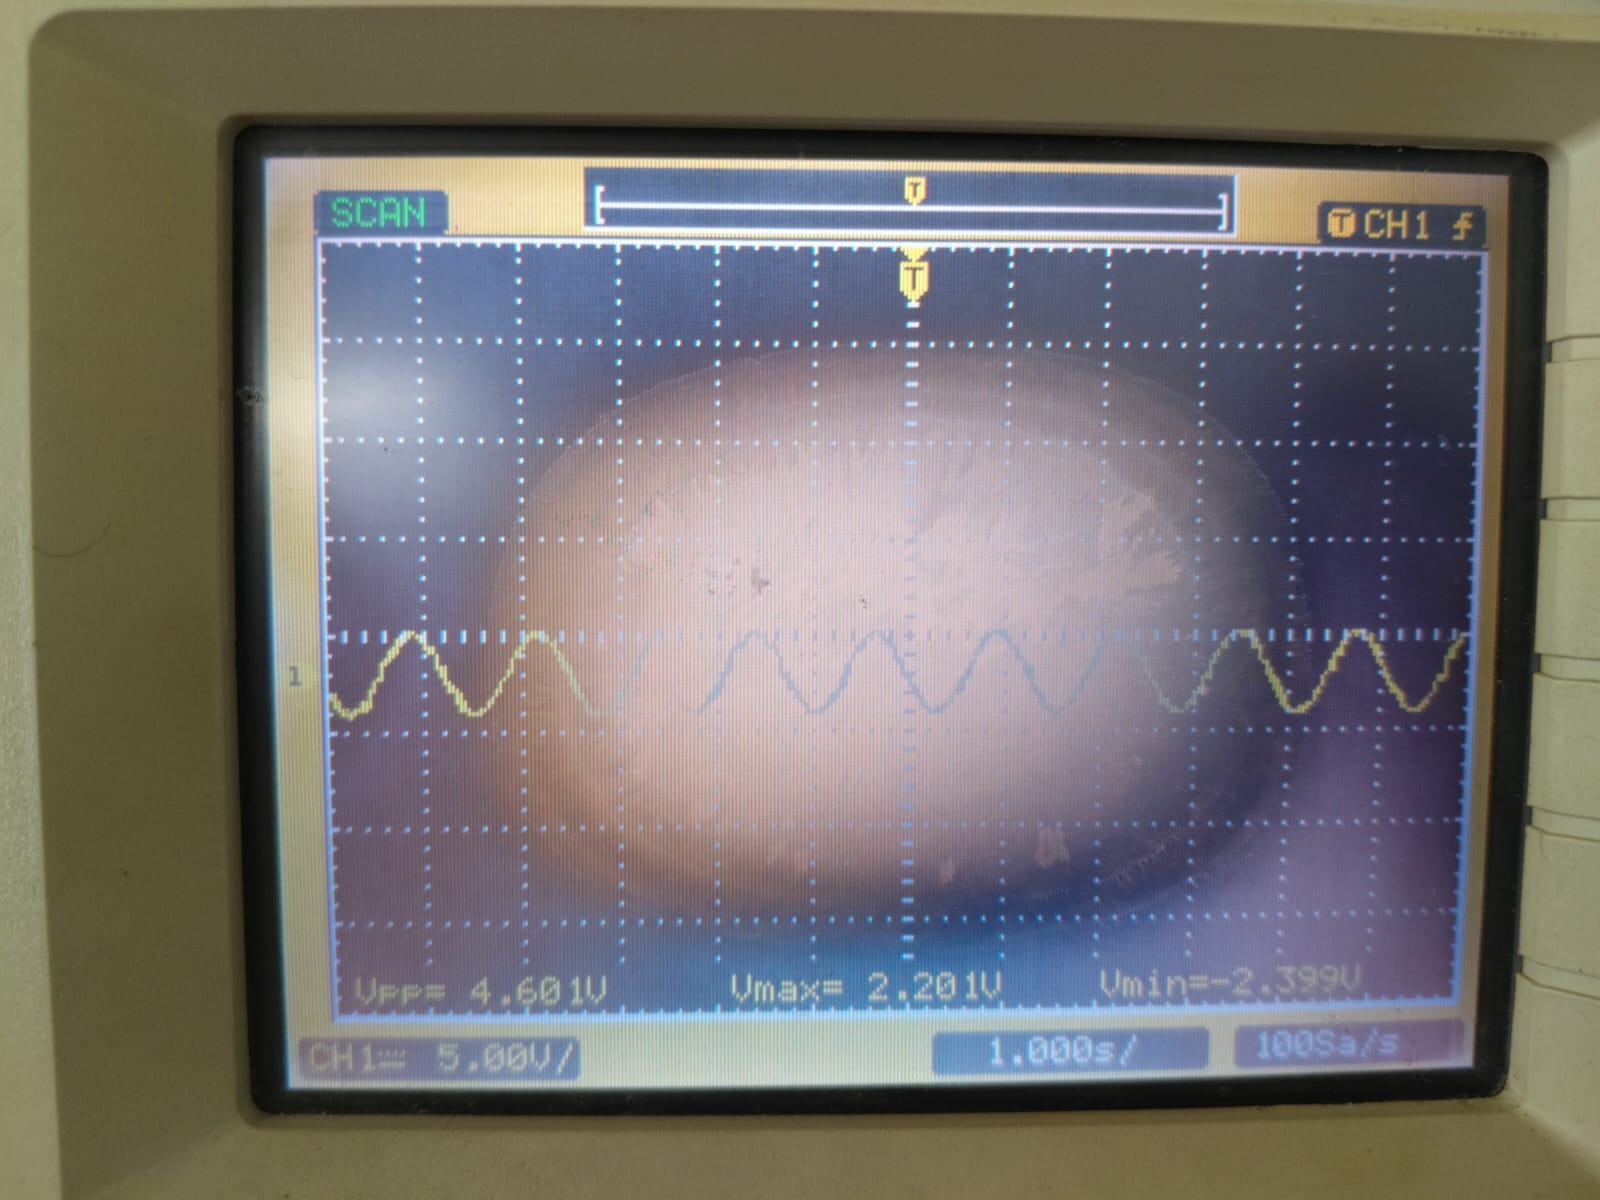
\includegraphics[width=\textwidth]{fig/hp/20ko.jpeg}
        \caption{Oscilloscope reading for frequency 20kHz}
        %\label{fig:image1}
    \end{minipage}
    \hfill
    \begin{minipage}[b]{0.45\textwidth}
        \centering
        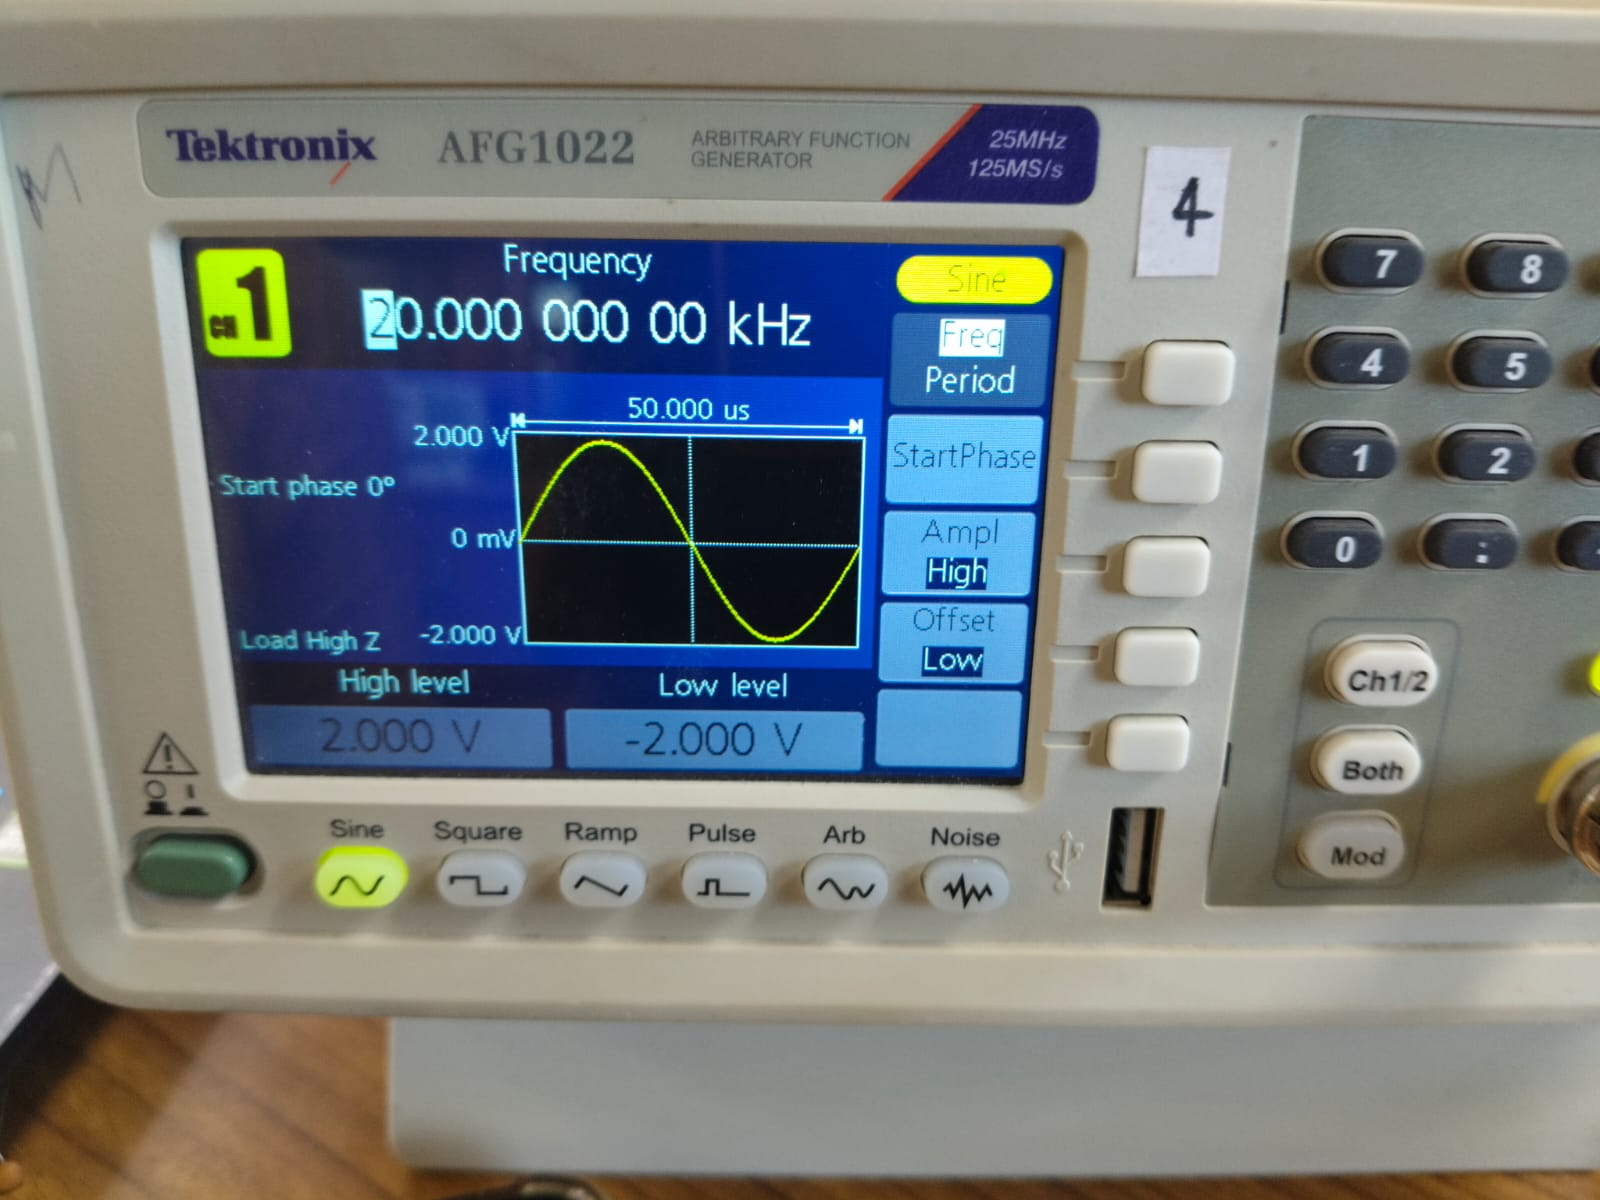
\includegraphics[width=\textwidth]{fig/hp/20k.jpeg}
        \caption{FG}
        %\label{fig:image2}
    \end{minipage}
\end{figure}
\subsubsection{Bode plot}

\begin{figure}[H]
    \centering
    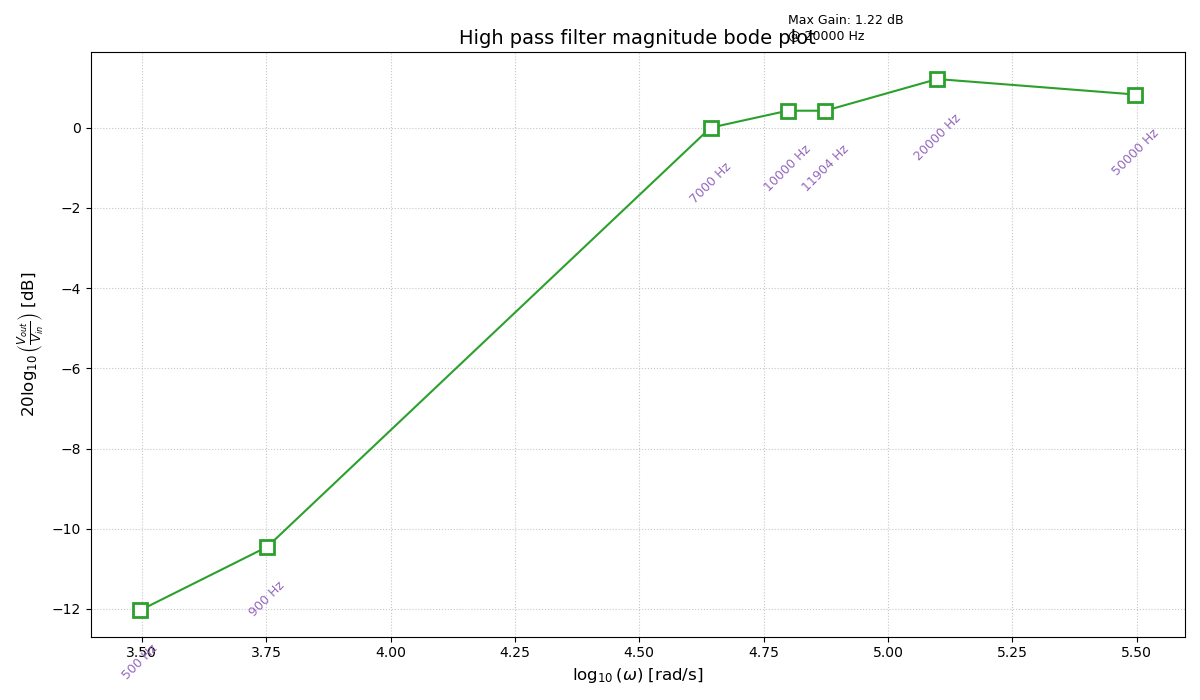
\includegraphics[width=0.8\textwidth]{fig/hpb.png}
    \caption{High pass BP- Measured}
    \label{fig:your-label}
\end{figure}

\begin{figure}[H]
    \centering
    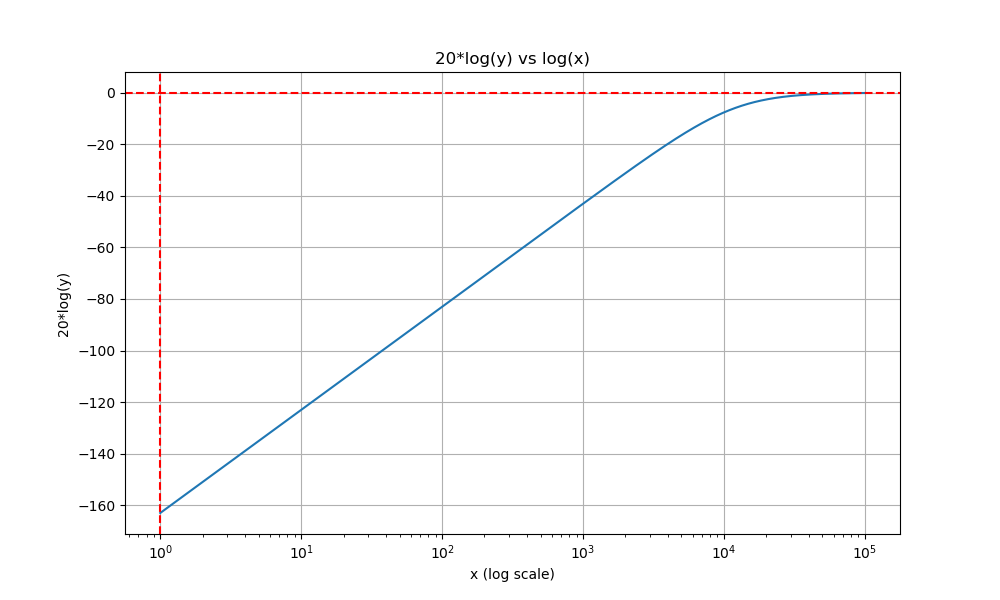
\includegraphics[width=0.8\textwidth]{hpfp.png}
    \caption{High pass BP- Theoretical}
    \label{fig:your-label}
\end{figure}

\subsection{Band-Pass fiter}
\begin{enumerate}
     \item Assemble the Sallen-key BPF circuit on the breadboard.
    \item Use the function Generator to apply a sine wave.
    \item Vary the input frequency and measure the output voltage.
    \item Record gain values for different frequencies.
    \item Plot gain vs. frequency (Bode plot). 
\end{enumerate}

\begin{figure}[H]
    \centering
    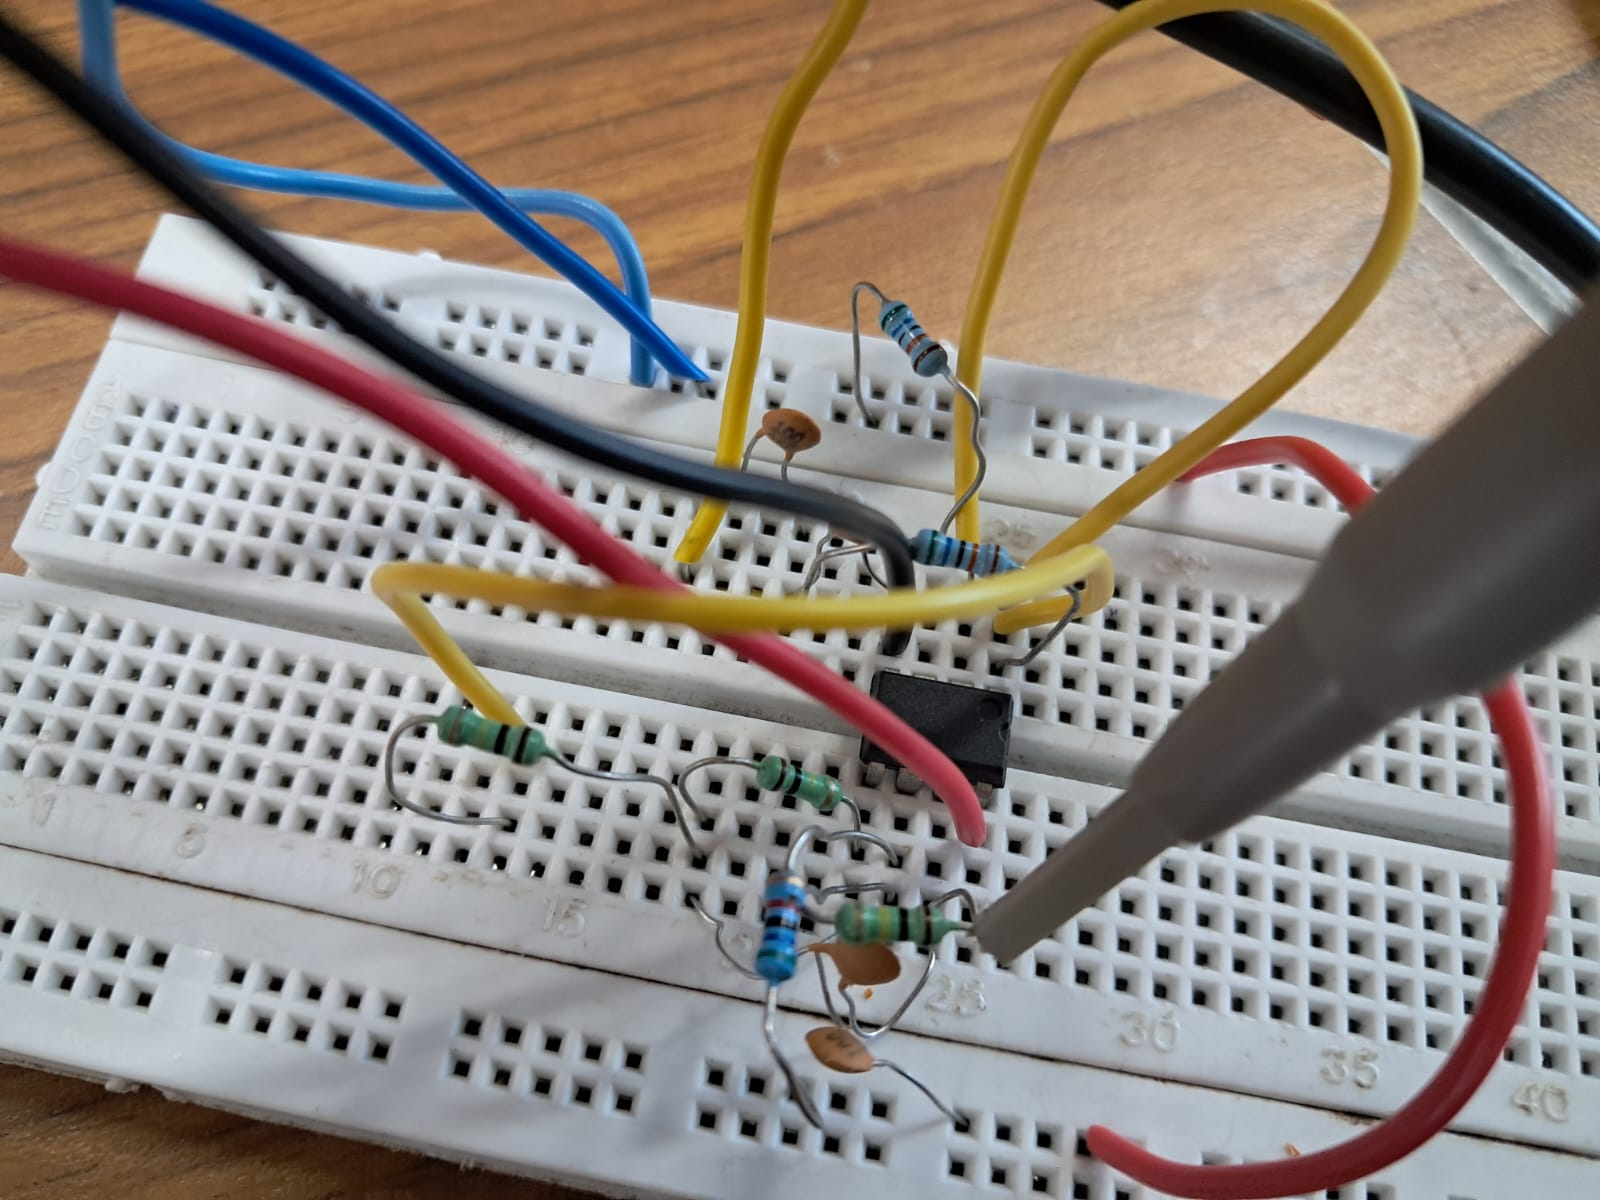
\includegraphics[width=0.8\textwidth]{fig/bp.jpeg}
    \caption{Circuit Diagram}
    \label{fig:your-label}
\end{figure}

\subsubsection{Observations}
\begin{table}[H]
\centering
\begin{tabular}{|c|c|c|}
\hline
\textbf{Frequency(in Hz)} & \textbf{Measured Value}  \\
\hline
2000 & 3.801    \\
3000& 5.801    \\
5000 & 7.801   \\
6000 & 8.001   \\
8000 & 7.601   \\
%9000 & 3.9 & \\
10000 & 7.201  \\
20000 & 4.601  \\
%7000 & 2.08 & 7.2 \\
%8000 & 1.58 & 8.3 \\
\hline
\end{tabular}
\caption{Measured vs Theoretical Values}
\end{table}
\begin{figure}[H]
    \centering
    \begin{minipage}[b]{0.45\textwidth}
        \centering
        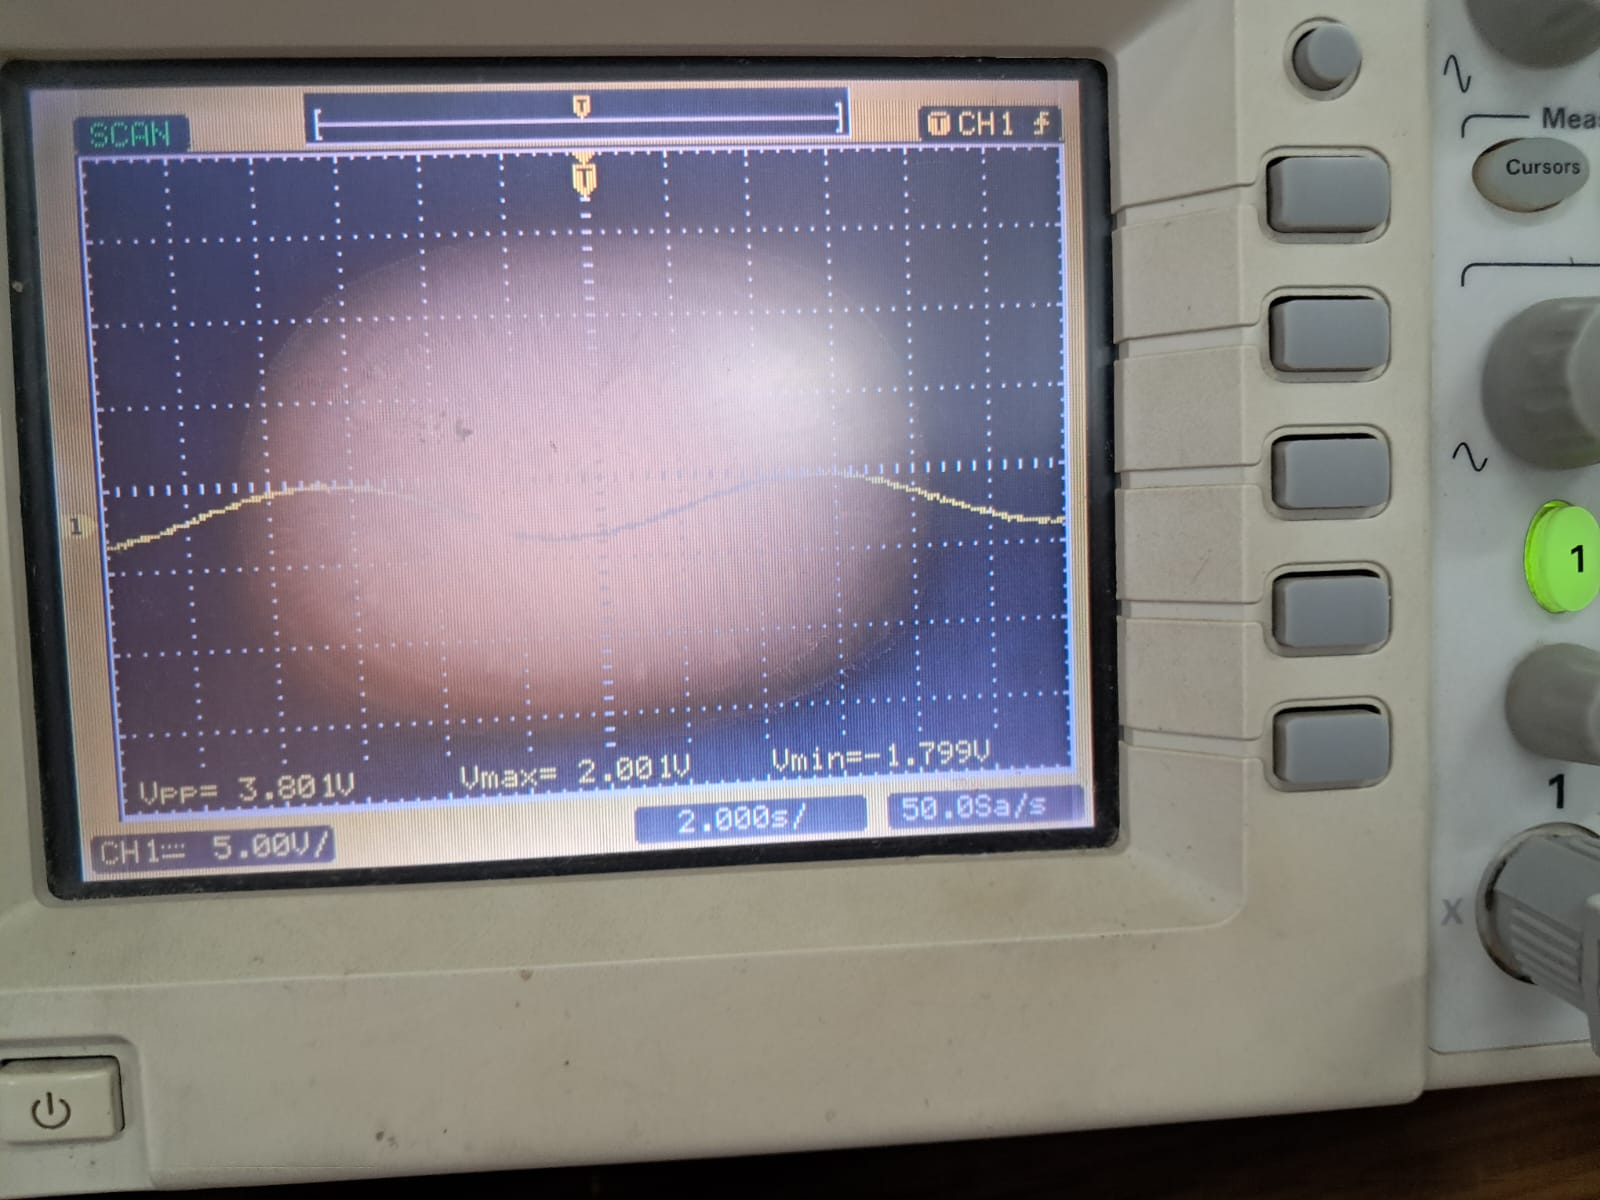
\includegraphics[width=\textwidth]{fig/bp/2ko.jpeg}
        \caption{Oscilloscope reading for frequency 2kHz}
        %\label{fig:image1}
    \end{minipage}
    \hfill
    \begin{minipage}[b]{0.45\textwidth}
        \centering
        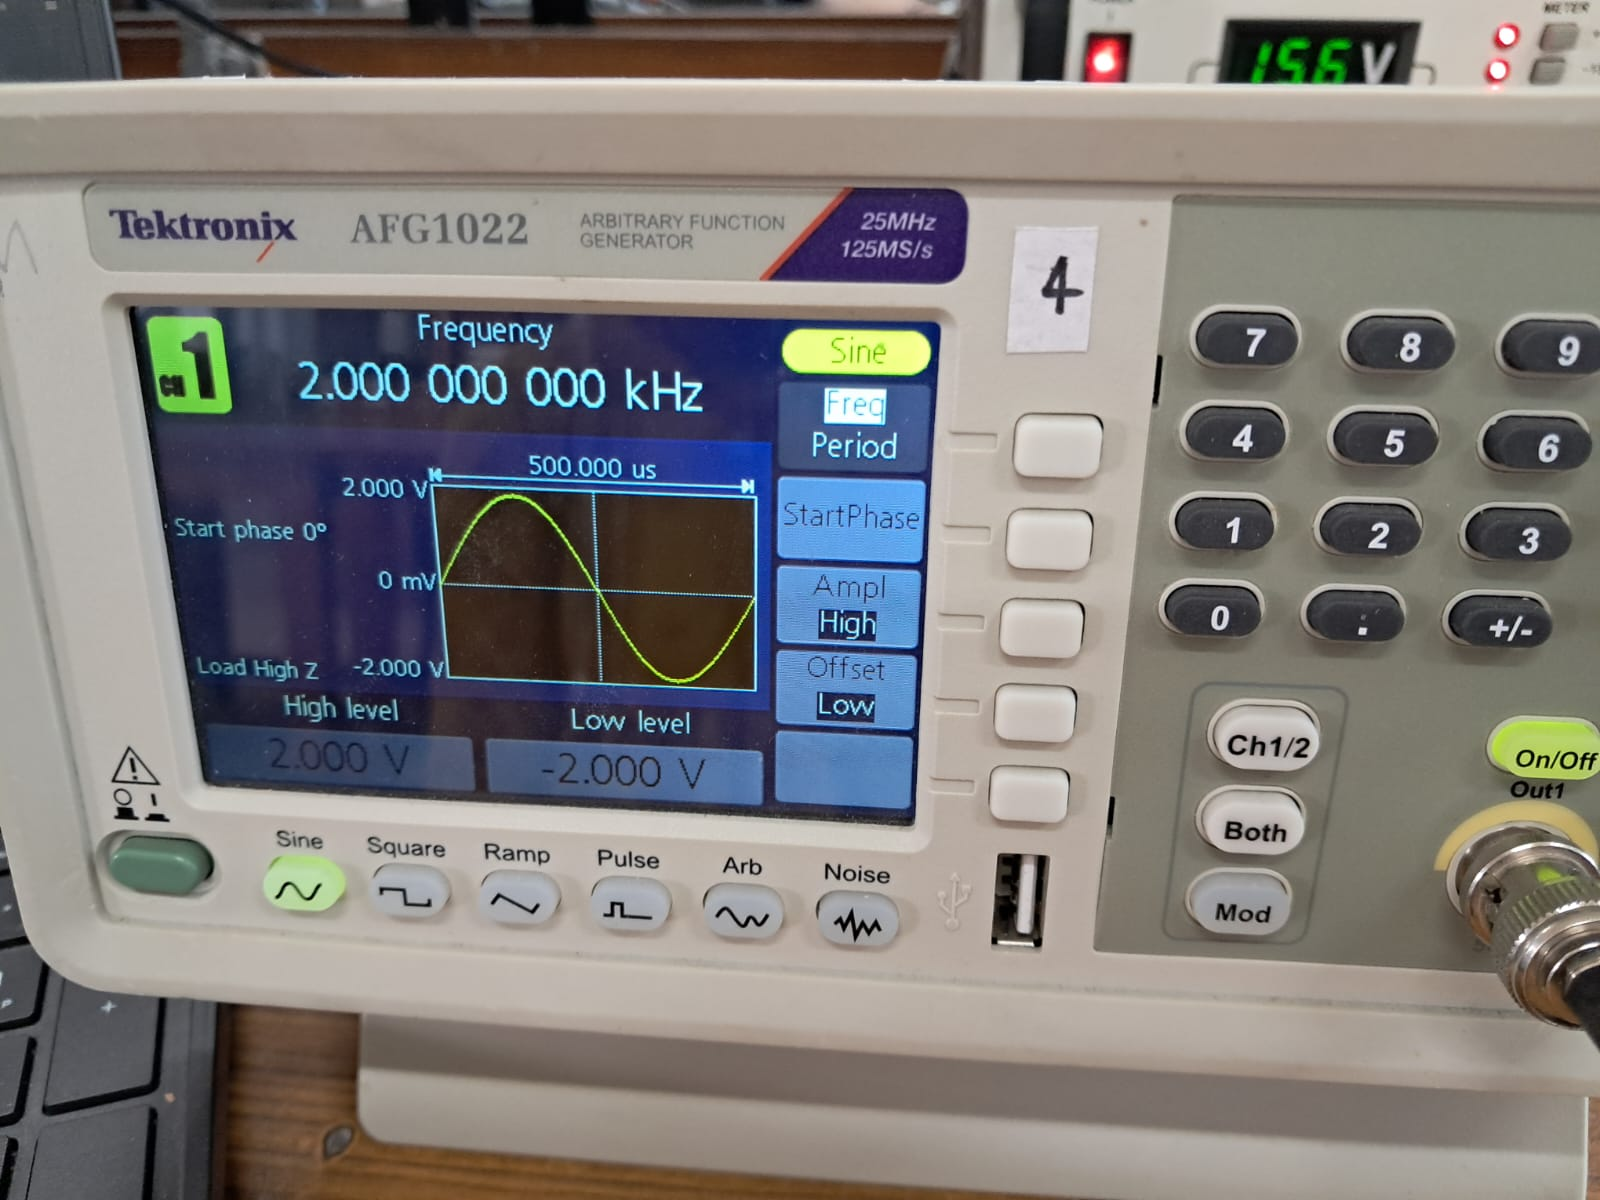
\includegraphics[width=\textwidth]{fig/bp/2k.jpeg}
        \caption{FG}
        %\label{fig:image2}
    \end{minipage}
\end{figure}

\begin{figure}[H]
    \centering
    \begin{minipage}[b]{0.45\textwidth}
        \centering
        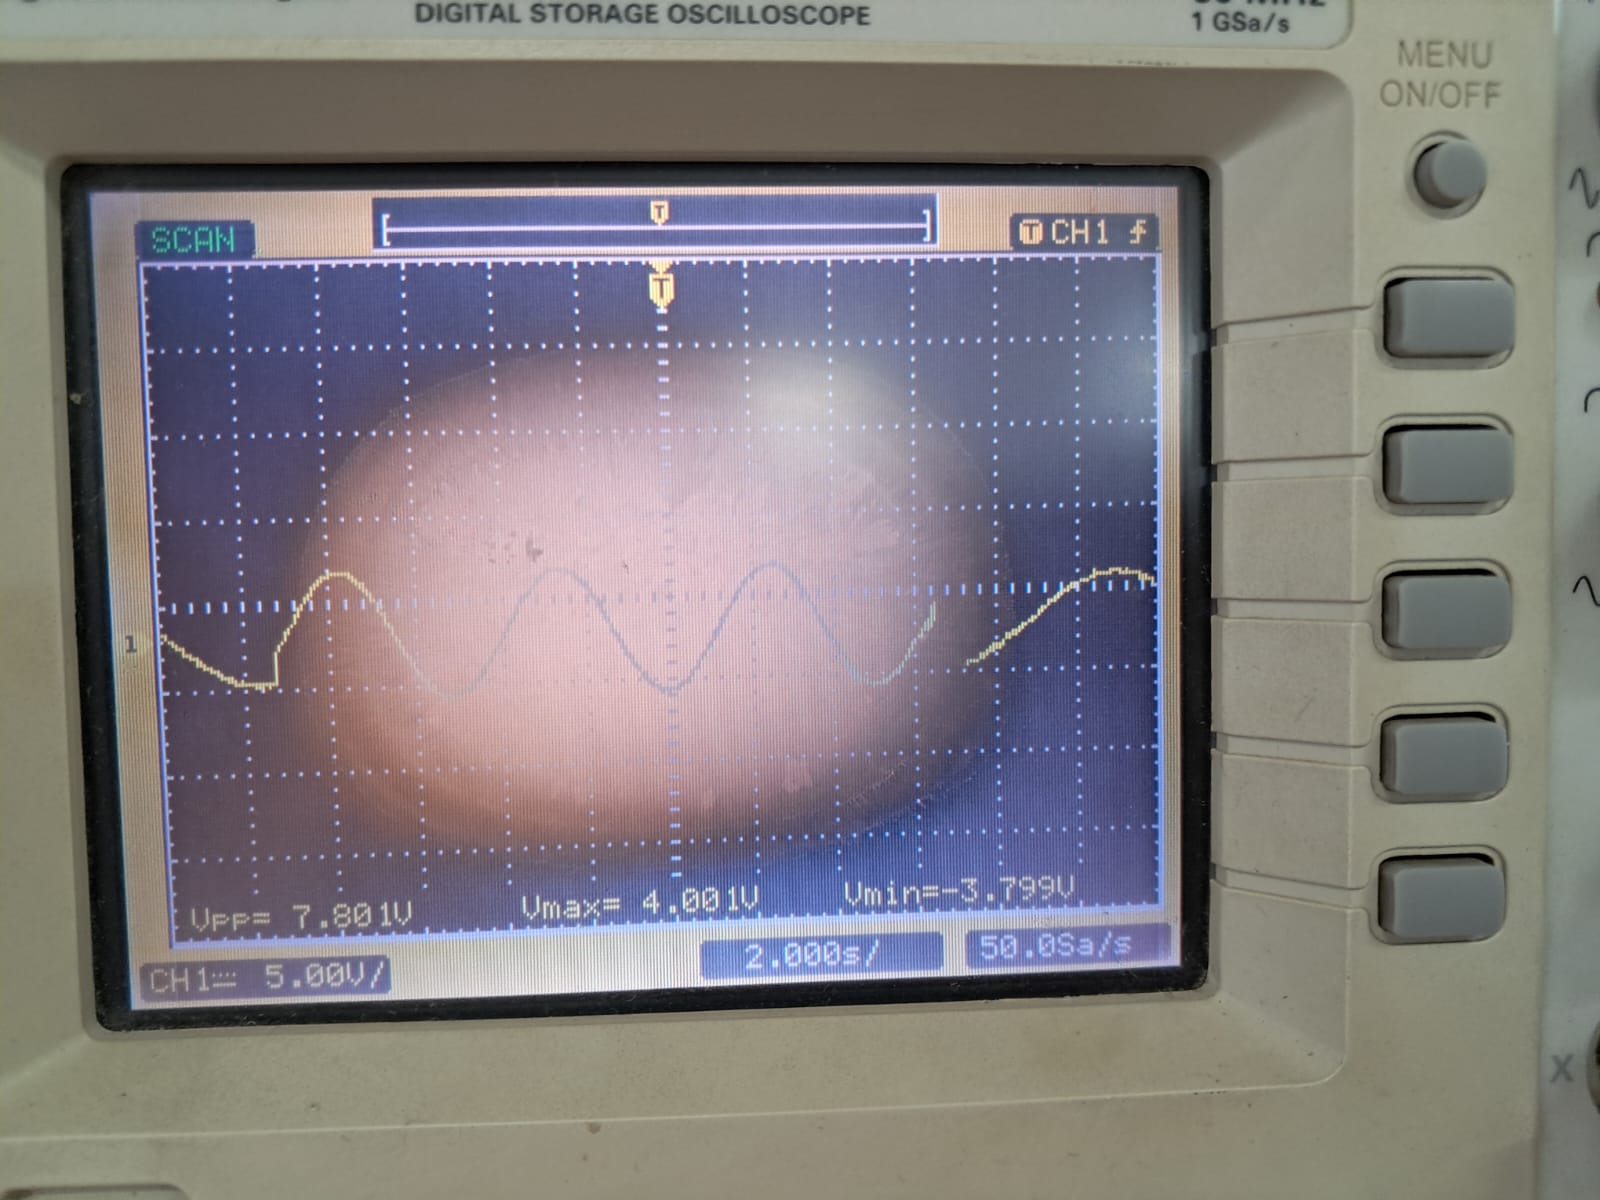
\includegraphics[width=\textwidth]{fig/bp/5ko.jpeg}
        \caption{Oscilloscope reading for frequency 5kHz}
        %\label{fig:image1}
    \end{minipage}
    \hfill
    \begin{minipage}[b]{0.45\textwidth}
        \centering
        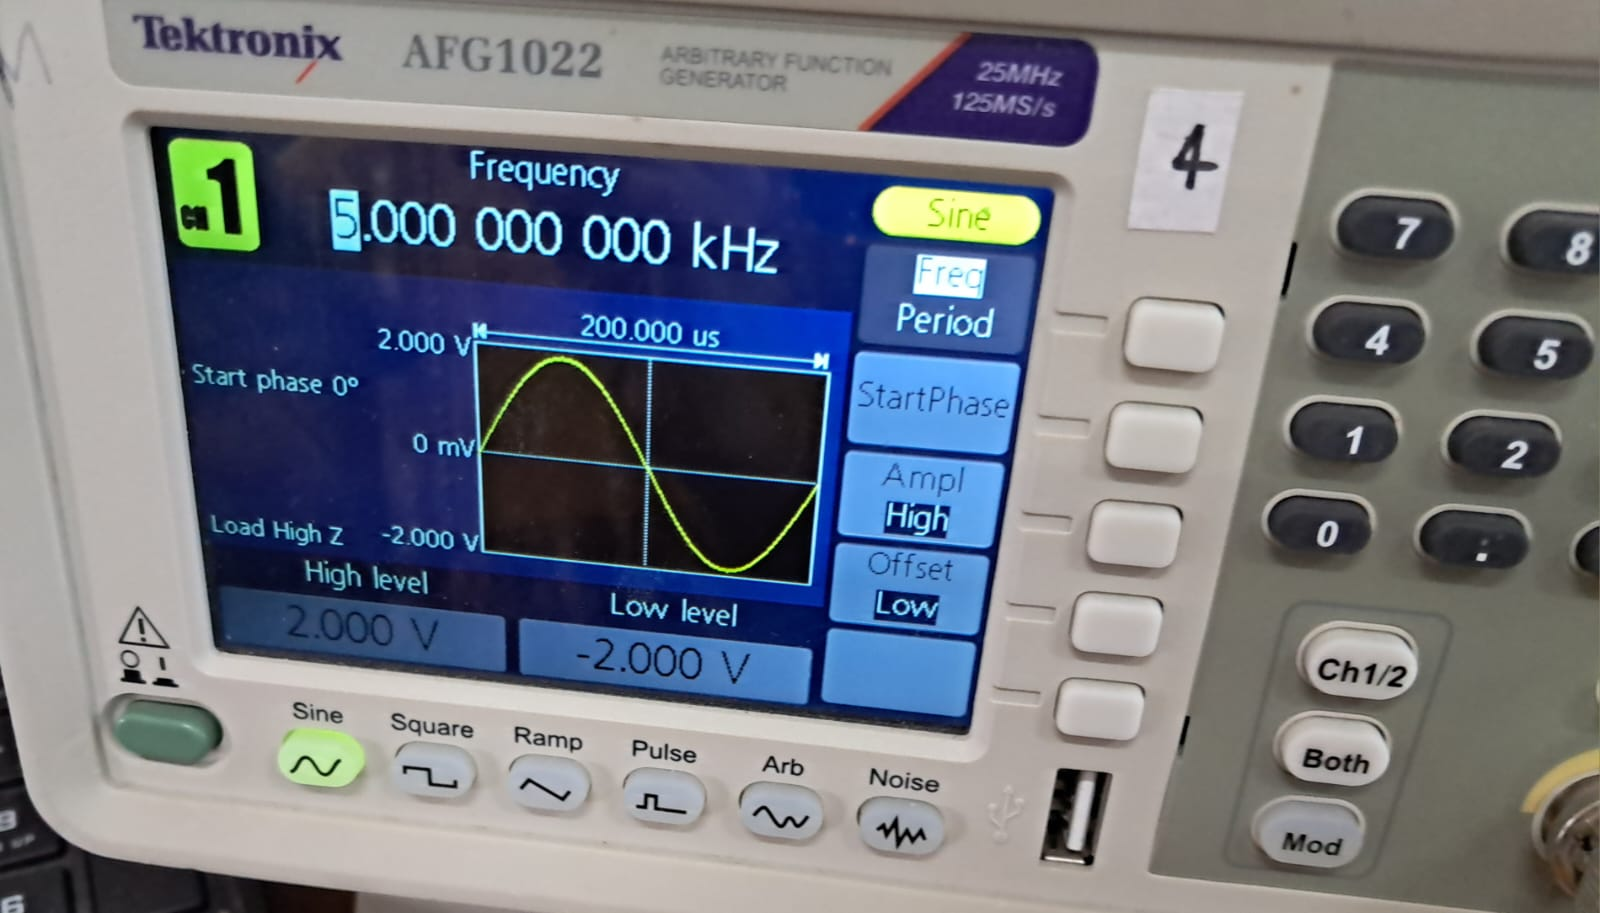
\includegraphics[width=\textwidth]{fig/bp/5k.jpeg}
        \caption{FG}
        %\label{fig:image2}
    \end{minipage}
\end{figure}

\begin{figure}[H]
    \centering
    \begin{minipage}[b]{0.45\textwidth}
        \centering
        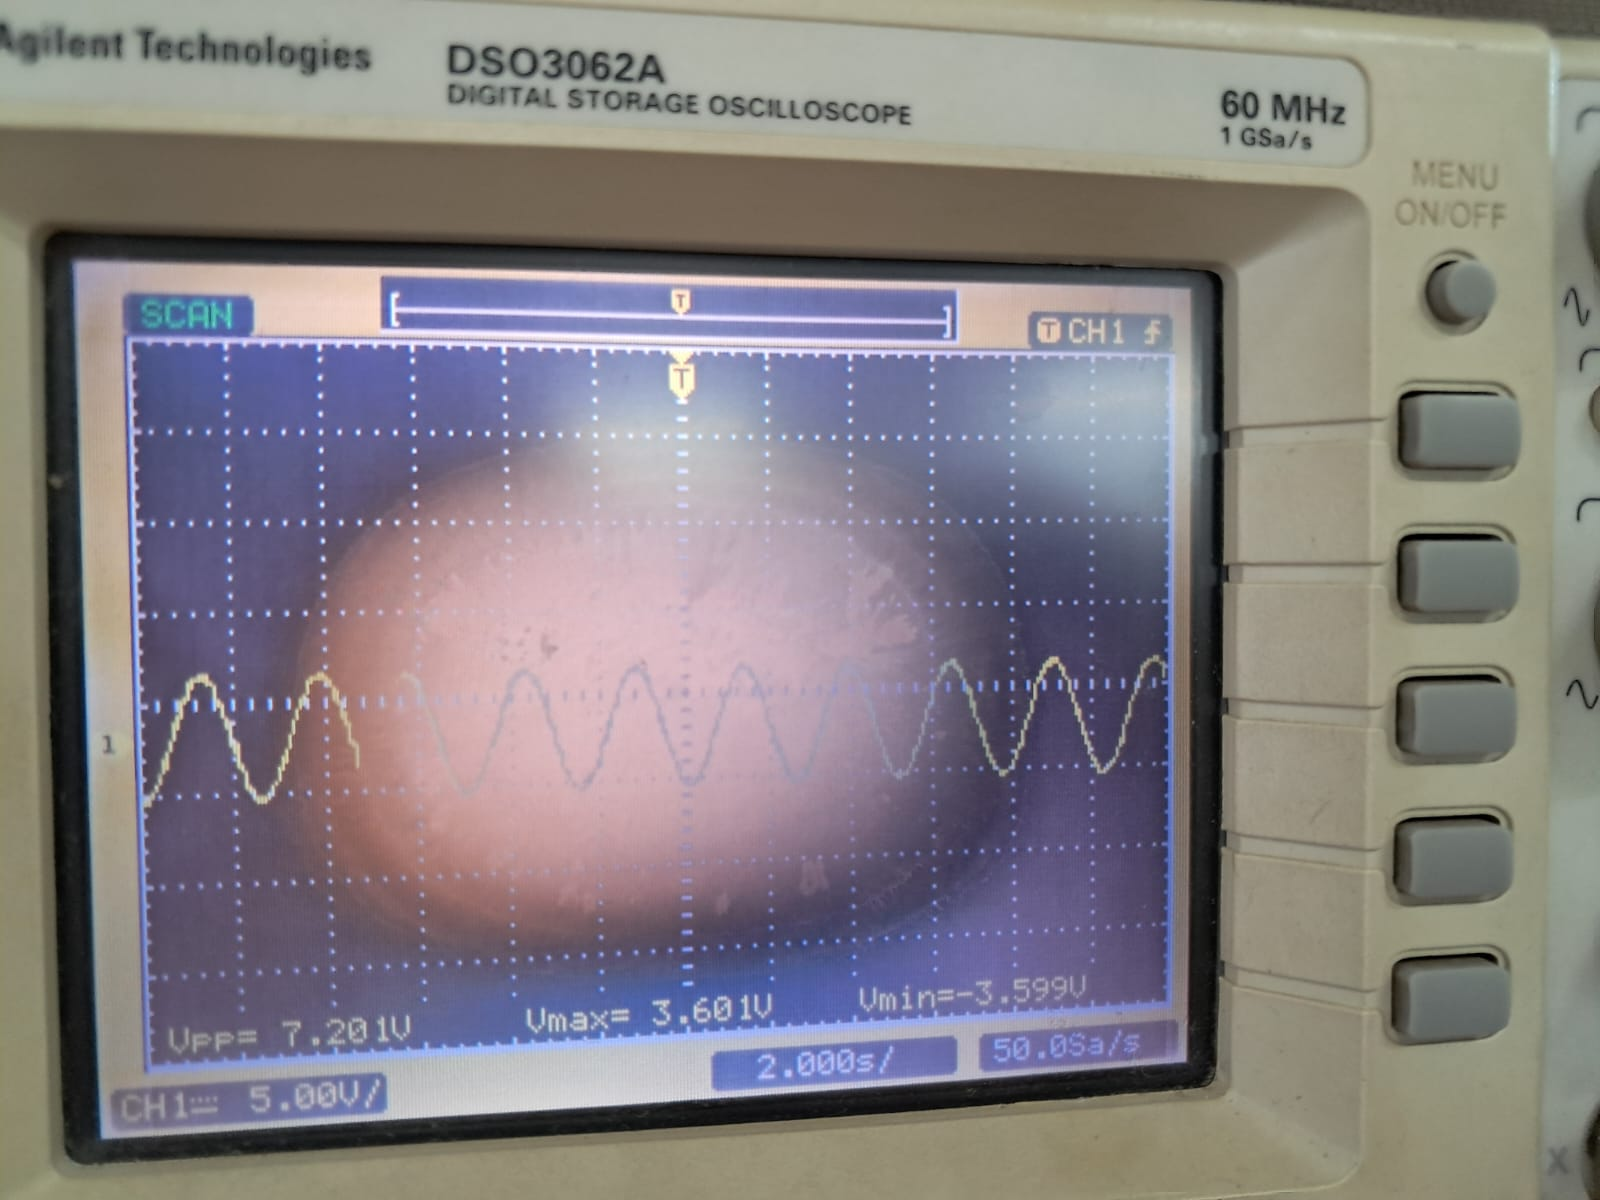
\includegraphics[width=\textwidth]{fig/bp/10ko.jpeg}
        \caption{Oscilloscope reading for frequency 10kHz}
        %\label{fig:image1}
    \end{minipage}
    \hfill
    \begin{minipage}[b]{0.45\textwidth}
        \centering
        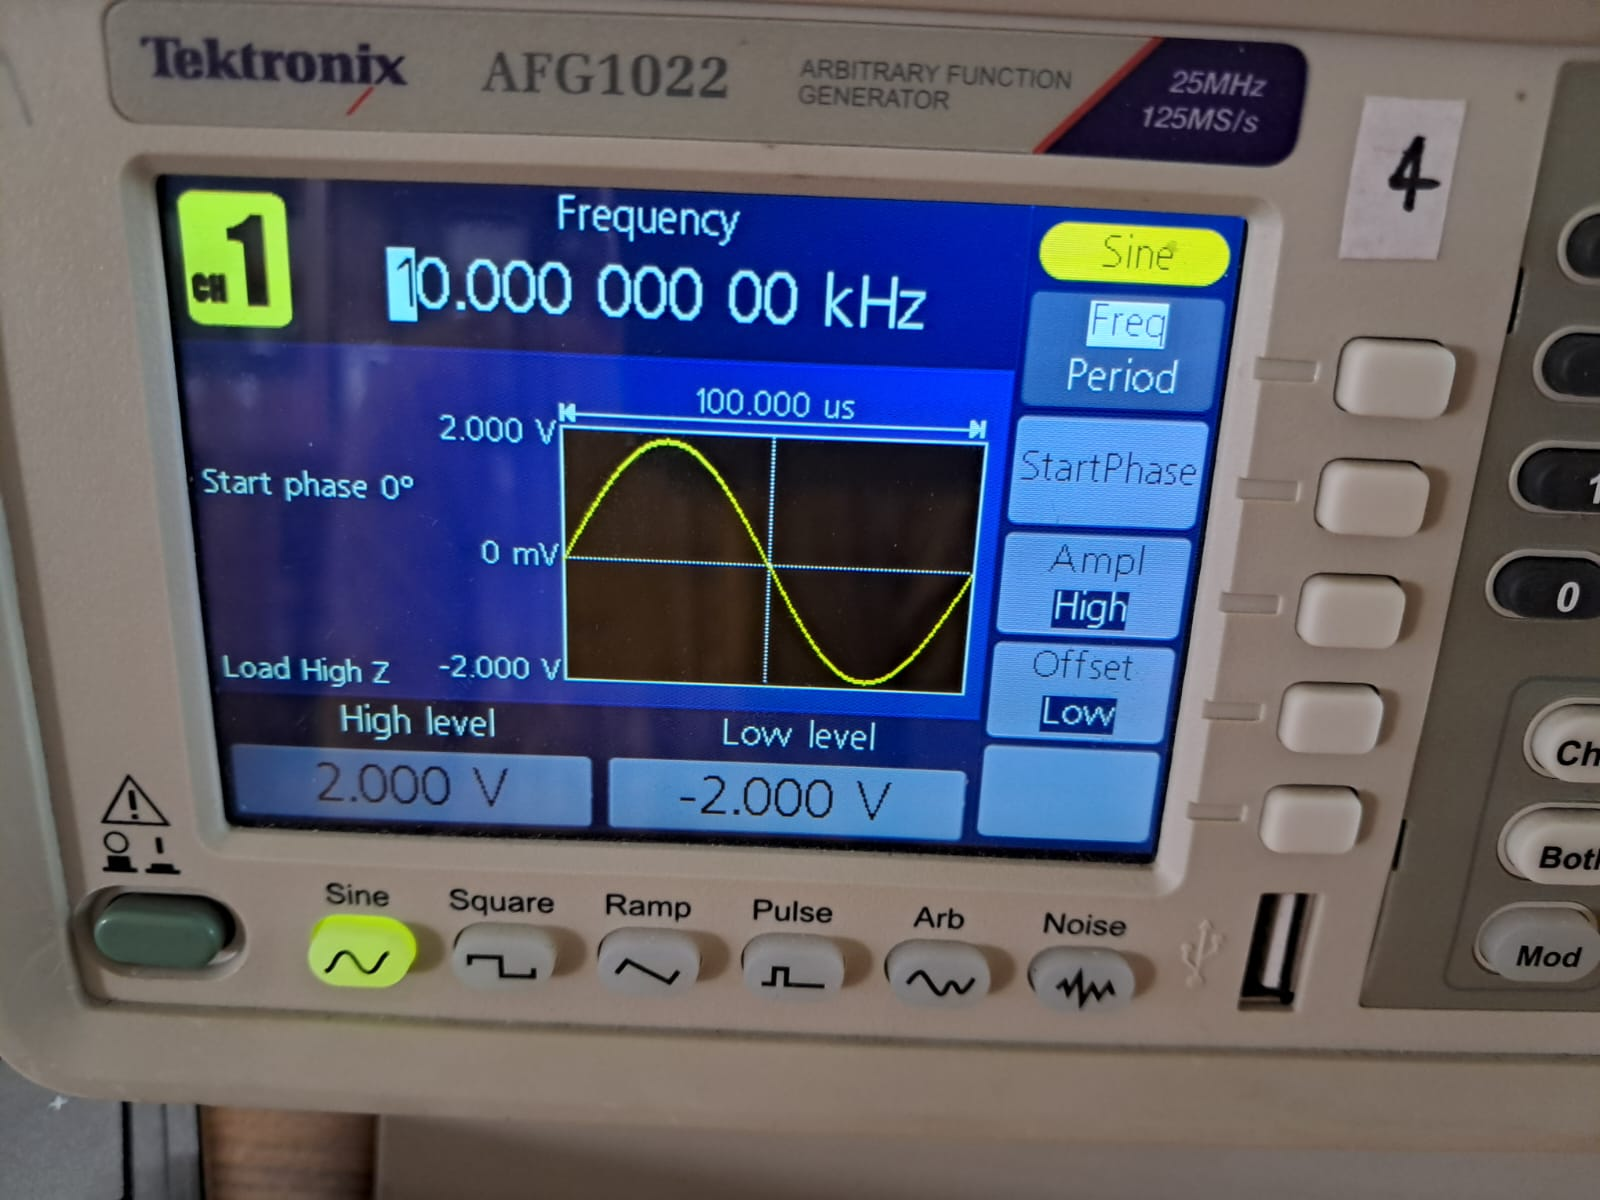
\includegraphics[width=\textwidth]{fig/bp/10k.jpeg}
        \caption{FG}
        %\label{fig:image2}
    \end{minipage}
\end{figure}

\begin{figure}[H]
    \centering
    \begin{minipage}[b]{0.45\textwidth}
        \centering
        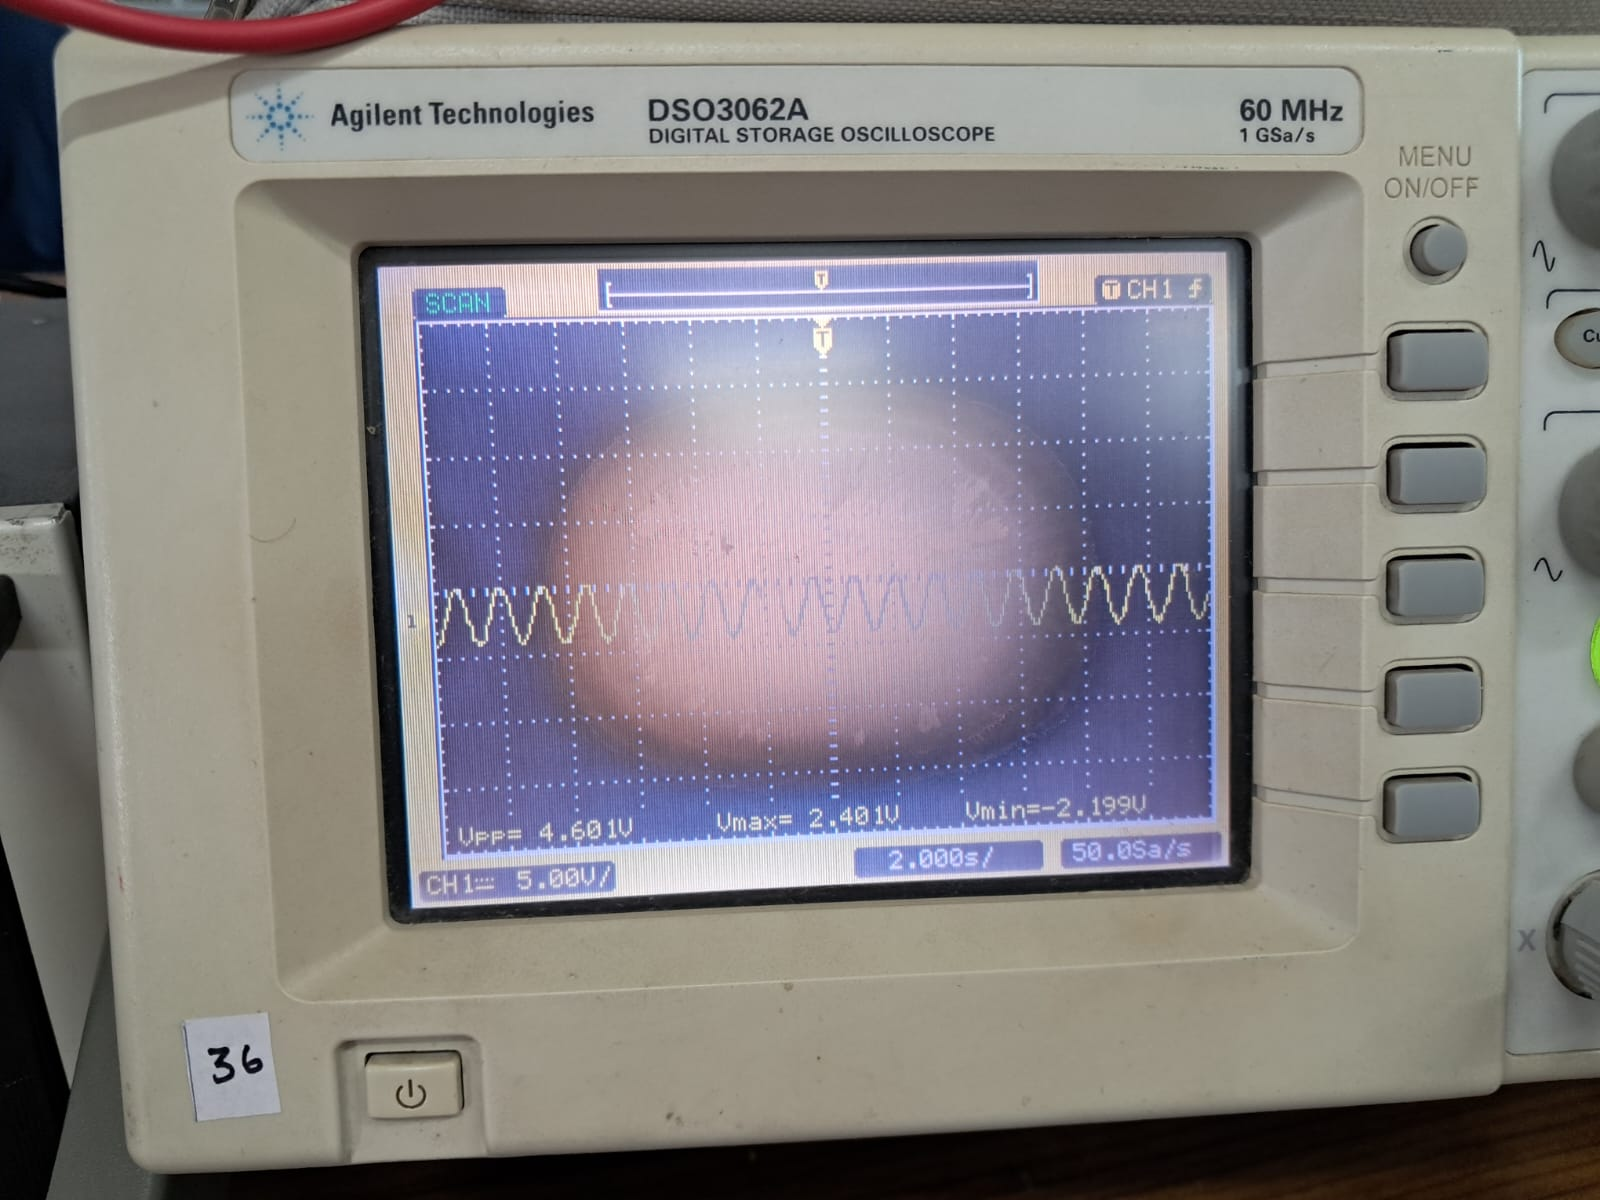
\includegraphics[width=\textwidth]{fig/bp/20ko.jpeg}
        \caption{Oscilloscope reading for frequency 20kHz}
        %\label{fig:image1}
    \end{minipage}
    \hfill
    \begin{minipage}[b]{0.45\textwidth}
        \centering
        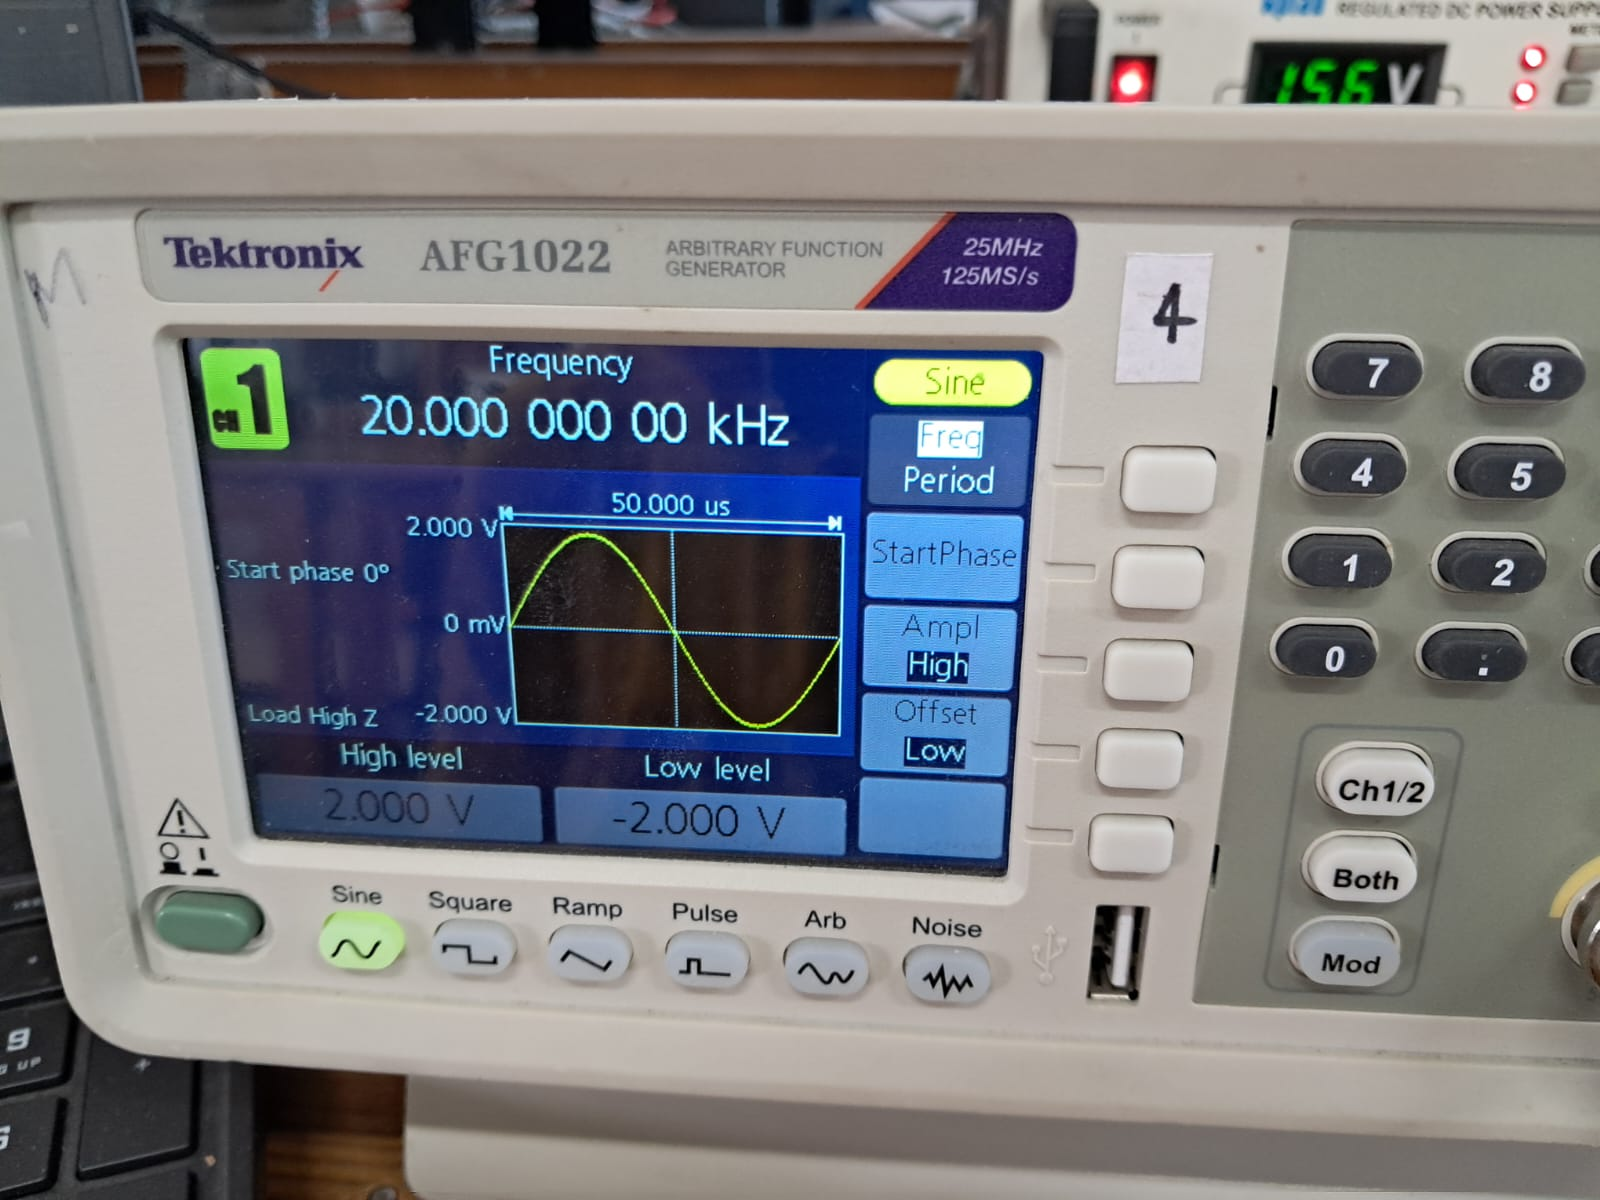
\includegraphics[width=\textwidth]{fig/bp/20k.jpeg}
        \caption{FG}
        %\label{fig:image2}
    \end{minipage}
\end{figure}

\section{Conclusion}
\begin{itemize}
    \item The experiment verifies the cascading method to form a bandpass filter.
    \item The experimental results match the theoretical calculations.
    \item Sallen-Key topology provide good stability and response.
\end{itemize}

\subsubsection{Bode plot}

\begin{figure}[H]
    \centering
    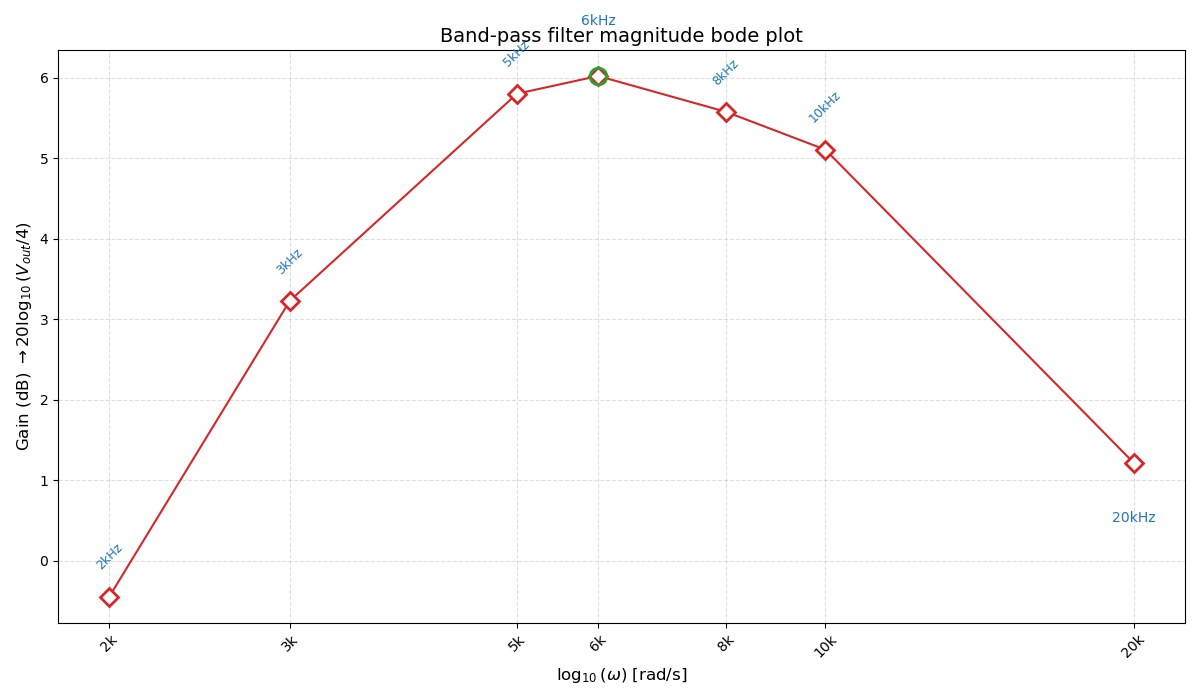
\includegraphics[width=0.8\textwidth]{fig/bpb.png}
    \caption{Band pass BP- Measured}
    \label{fig:your-label}
\end{figure}

\begin{figure}[H]
    \centering
    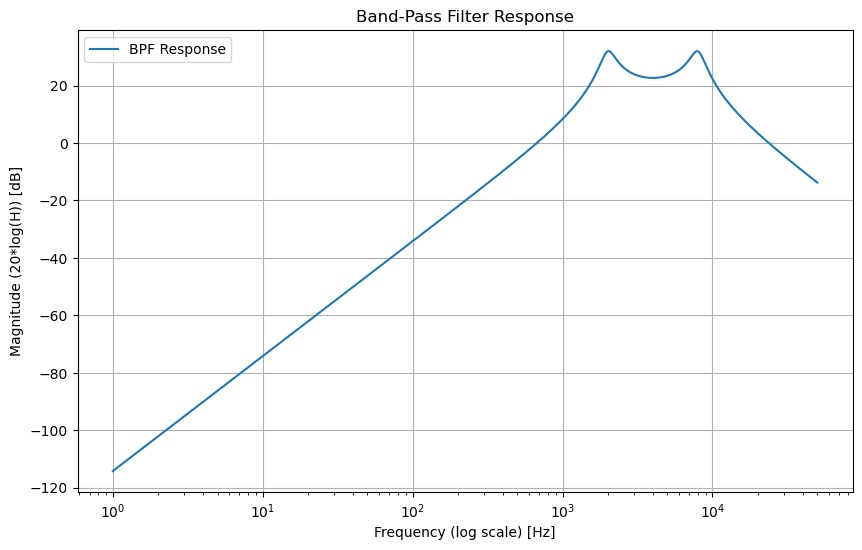
\includegraphics[width=0.8\textwidth]{bpfp.jpeg}
    \caption{Band pass BP- Theoretical}
    \label{fig:your-label}
\end{figure}


\end{document}
